\chapter{Results}
\label{chap:results}

\begin{figure}[htbp]
    \centering
    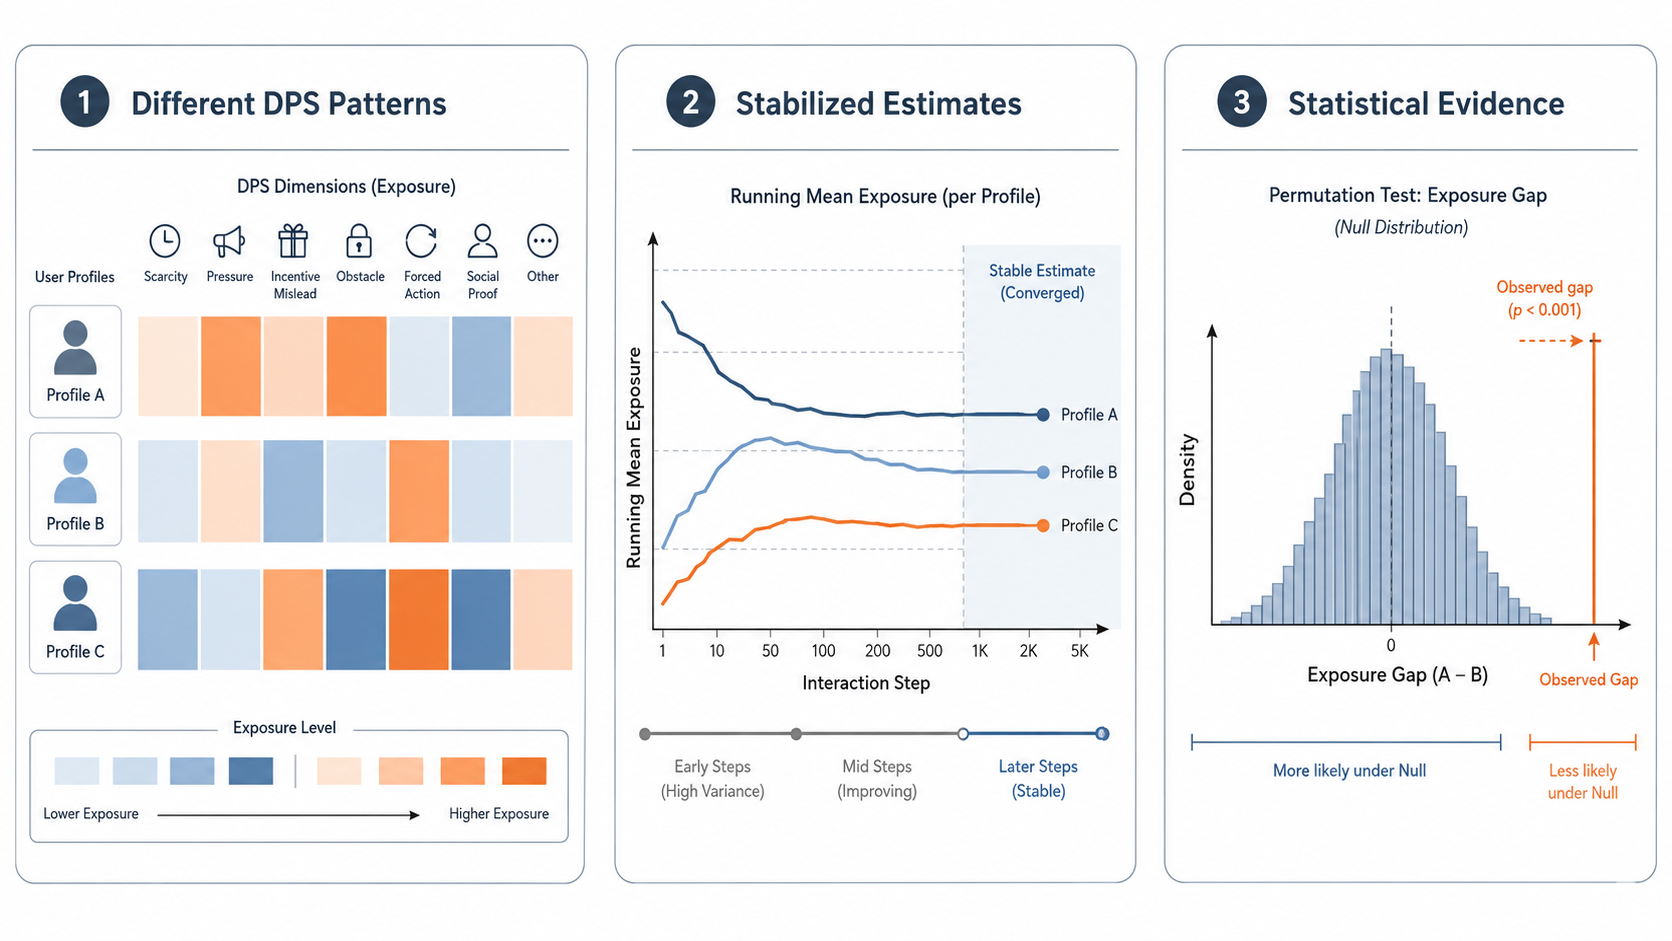
\includegraphics[width=0.95\linewidth]{figures/pictures/results_dashboard_overview.png}
    \caption{Dashboard Overview}
    \label{fig:dashboard_overview}
\end{figure}


\section{Overview of Results}

This section reports the empirical results of the profile-aware dark pattern auditing experiment. The repository contains 1,403 interaction records from 16 mobile applications and three controlled user profiles. The protocol was designed around 30 interaction steps for each app-profile pair; in the archived results, the observed trajectory length ranges from 20 to 30 steps because a small number of runs ended before the planned length. Since each interaction record was annotated with the seven-dimensional DPS vector, the resulting dataset contains 9,821 dimension-level DPS labels. These labels provide the basis for estimating profile-conditioned dark pattern exposure, comparing exposure differences across profiles, and examining whether observed differences are likely to reflect systematic profile-dependent variation rather than random fluctuation.

\begin{table}[htbp]
    \centering
    \caption{Summary of the experimental result dataset.}
    \label{tab:results-overview}
    \begin{tabular}{ll}
        \toprule
        Item & Value \\
        \midrule
        Number of apps & 16 \\
        Number of profiles & 3 \\
        Steps per app-profile pair & Planned: 30; observed: 20--30 \\
        Total interaction records & 1,403 \\
        Total DPS labels & 9,821 \\
        DPS dimensions & I, F, P, C, S, N, FA \\
        \bottomrule
    \end{tabular}
\end{table}

Overall, the results suggest that dark pattern exposure is not uniform across controlled user profiles. Different profiles produce visibly different DPS distributions, and these differences appear across multiple forms of analysis. The heatmaps show that the average exposure intensity varies not only across applications and app categories, but also across user profiles. The running mean convergence curves further indicate that exposure estimates gradually stabilize as interaction steps accumulate, suggesting that the results are not driven by isolated screenshots or single-step observations. Finally, the statistical validation metrics, including Mann-Whitney U q-values, permutation tests, L1 distance, and Cramér's V, provide converging evidence that profile type is associated with measurable differences in dark pattern exposure.

The main empirical pattern is that commercially oriented profiles, especially the high-payment shopping profile and the bargain-hunter profile, tend to encounter stronger exposure in dimensions related to interface interference and pressure. This does not imply that platforms deliberately single out those profiles with dark patterns. A more cautious interpretation is that profile-conditioned behavior changes the interaction trajectory, and different trajectories lead users into different interface regions where dark patterns are more or less likely to appear. For example, a user who frequently enters purchase, membership, coupon, or payment interfaces naturally observes more decision-stage interface designs than a user who mainly browses information feeds. In this sense, the results support the central claim of this project: dark pattern exposure should be analyzed as a profile-conditioned distribution along interaction trajectories, rather than as a static property of an application.

\section{Finding 1: Different Profiles Show Different DPS Patterns}

\paragraph{Result.}
The three controlled profiles show different DPS exposure patterns. At the aggregate level, the high-payment shopping profile has the highest mean DPS exposure, followed by the bargain-hunter profile and the low-payment browsing profile. The difference is not uniform across dimensions: the largest profile-level changes appear in Interface Interference, Pressure, and Forced Action, while Contextual Deception and Sneaking remain comparatively low in the overall dataset.
However, simply looking at the overall averages is not sufficiently distinctive on its own. The profile gap becomes much clearer when the analysis is broken down by application category, especially in social and food-delivery applications.

\begin{table}[htbp]
    \centering
    \caption{Profile-level mean DPS exposure across all audited applications.}
    \label{tab:profile-mean-dps}
    \footnotesize
    \begin{tabular}{lrrrrrrrr}
        \toprule
        Profile & I & F & P & C & S & N & FA & Total / Mean \\
        \midrule
        High-payment shopping & 0.638 & 0.165 & 0.522 & 0.030 & 0.030 & 0.163 & 0.717 & 2.264 / 0.323 \\
        Low-payment browsing & 0.518 & 0.130 & 0.477 & 0.022 & 0.028 & 0.117 & 0.672 & 1.963 / 0.280 \\
        Bargain hunter & 0.606 & 0.173 & 0.475 & 0.051 & 0.015 & 0.135 & 0.704 & 2.161 / 0.309 \\
        \bottomrule
    \end{tabular}%
\end{table}

\paragraph{Evidence.}
Table~\ref{tab:profile-mean-dps} reports the mean DPS values computed from the archived step-level CSV files. Figure~\ref{fig:mean-exposure-all} provides the corresponding heatmap. In this heatmap, rows represent controlled profiles and columns represent the seven DPS dimensions: Interface Interference, Friction, Pressure, Contextual Deception, Sneaking, Nagging, and Forced Action. The color intensity of each cell represents the average exposure score for a profile-dimension combination. A darker or more saturated cell therefore indicates stronger average exposure in that DPS dimension under a particular profile condition.

\begin{figure}[htbp]
    \centering
    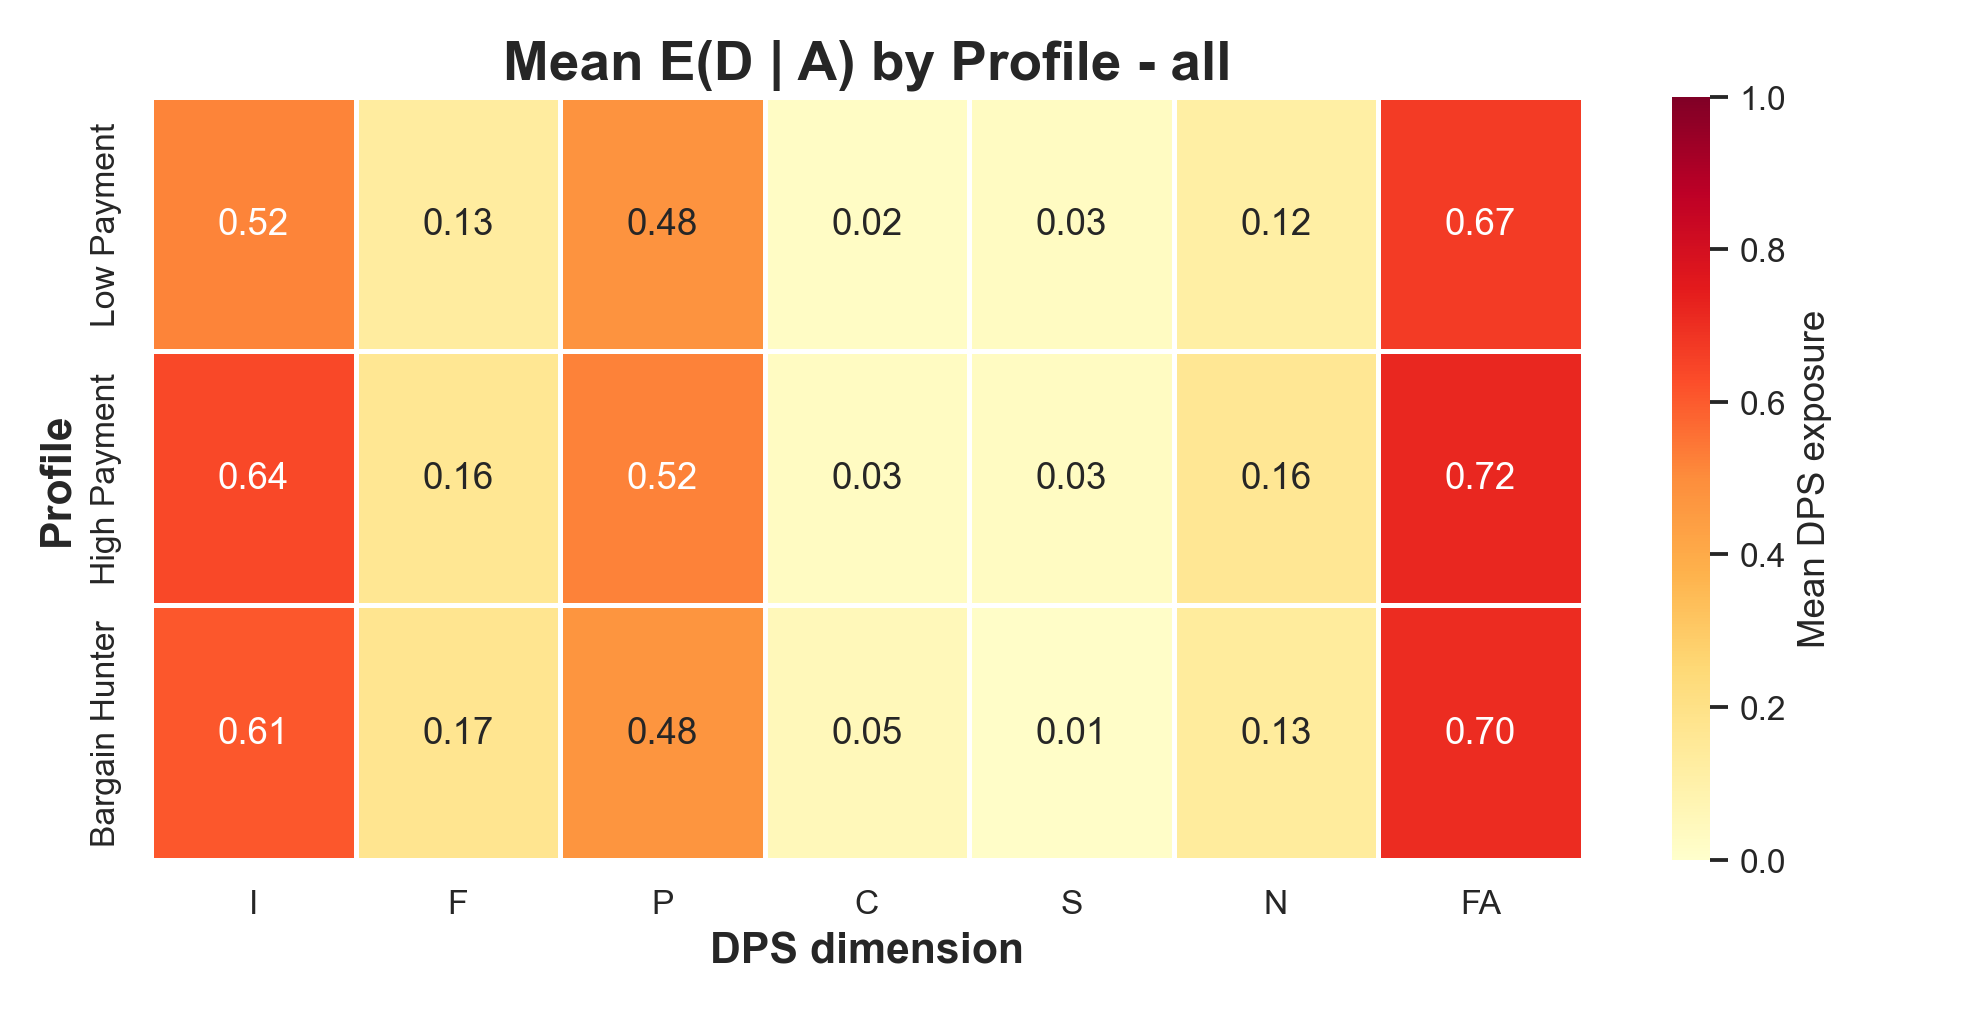
\includegraphics[width=0.95\linewidth]{figures/statistics/heatmap_mean_exposure_all.png}
    \caption{Mean DPS exposure across all audited applications and controlled profiles.}
    \label{fig:mean-exposure-all}
\end{figure}

\paragraph{Food-delivery evidence.}
The category-level result for food-delivery applications shows a clearer profile gap than the global average alone. Table~\ref{tab:eating-mean-dps} summarizes the mean DPS exposure for the food-delivery category across all audited applications in that scope. Figure~\ref{fig:mean-exposure-eating} shows the corresponding heatmap, where the separation between profiles is especially visible in Pressure and Forced Action.

\begin{table}[htbp]
    \centering
    \caption{Profile-level mean DPS exposure for food-delivery applications.}
    \label{tab:eating-mean-dps}
    \footnotesize
    \begin{tabular}{lrrrrrrrr}
        \toprule
        Profile & I & F & P & C & S & N & FA & Total / Mean \\
        \midrule
        High-payment shopping & 0.442 & 0.058 & 0.542 & 0.000 & 0.033 & 0.183 & 0.975 & 2.233 / 0.319 \\
        Low-payment browsing & 0.242 & 0.092 & 0.600 & 0.000 & 0.008 & 0.108 & 0.825 & 1.875 / 0.268 \\
        Bargain hunter & 0.442 & 0.100 & 0.483 & 0.000 & 0.000 & 0.075 & 0.925 & 2.025 / 0.289 \\
        \bottomrule
    \end{tabular}%
\end{table}

\begin{figure}[htbp]
    \centering
    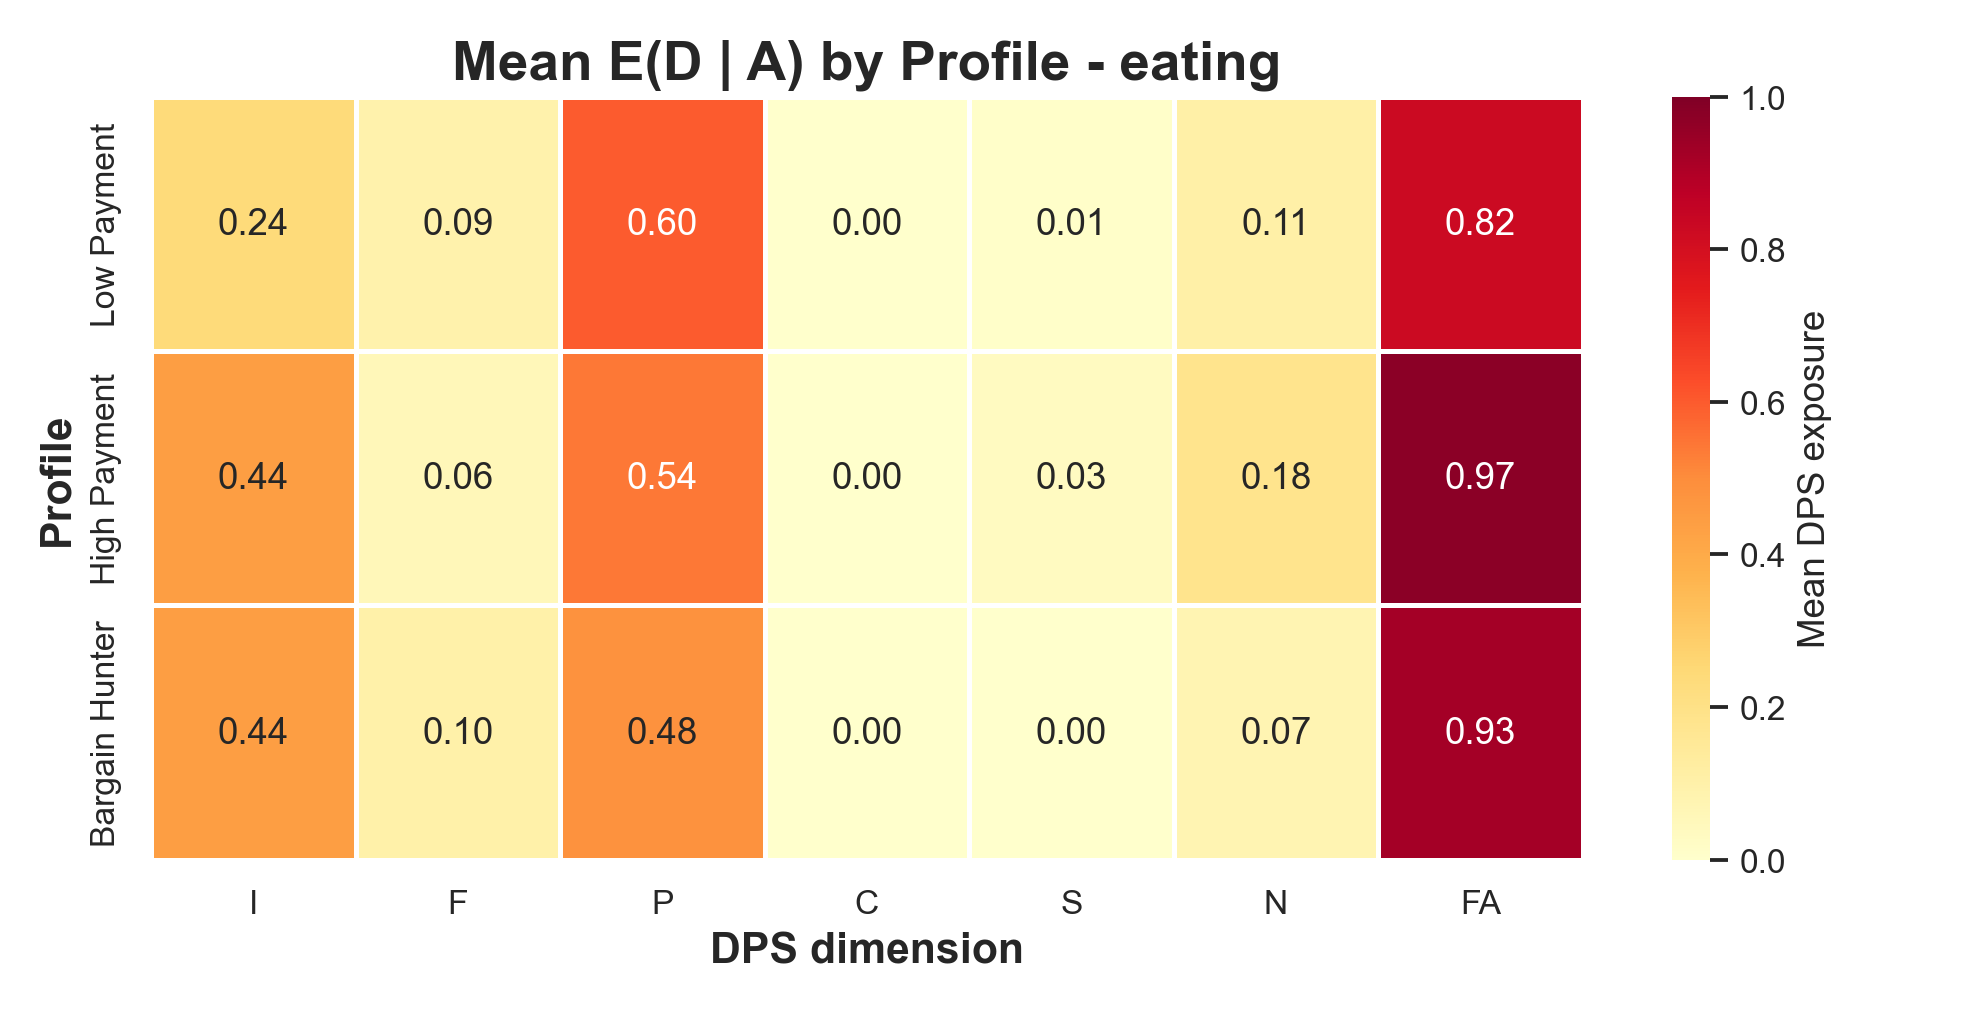
\includegraphics[width=0.95\linewidth]{figures/statistics/heatmap_mean_exposure_eating.png}
    \caption{Mean DPS exposure heatmap for food-delivery and eating-related applications.}
    \label{fig:mean-exposure-eating}
\end{figure}

\paragraph{Social evidence.}
Social applications show the clearest category-level separation among the audited domains. Table~\ref{tab:social-mean-dps} summarizes the mean DPS exposure for social applications across the audited sample. Figure~\ref{fig:mean-exposure-social} shows the corresponding heatmap, where Interface Interference, Friction, and Nagging differ visibly across profiles.

\begin{table}[htbp]
    \centering
    \caption{Profile-level mean DPS exposure for social applications.}
    \label{tab:social-mean-dps}
    \footnotesize
    \begin{tabular}{lrrrrrrrr}
        \toprule
        Profile & I & F & P & C & S & N & FA & Total / Mean \\
        \midrule
        High-payment shopping & 1.319 & 0.451 & 0.504 & 0.053 & 0.053 & 0.389 & 0.044 & 2.814 / 0.402 \\
        Low-payment browsing & 0.958 & 0.250 & 0.333 & 0.083 & 0.100 & 0.242 & 0.083 & 2.050 / 0.293 \\
        Bargain hunter & 1.089 & 0.384 & 0.473 & 0.161 & 0.045 & 0.286 & 0.080 & 2.473 / 0.353 \\
        \bottomrule
    \end{tabular}%
\end{table}

\begin{figure}[htbp]
    \centering
    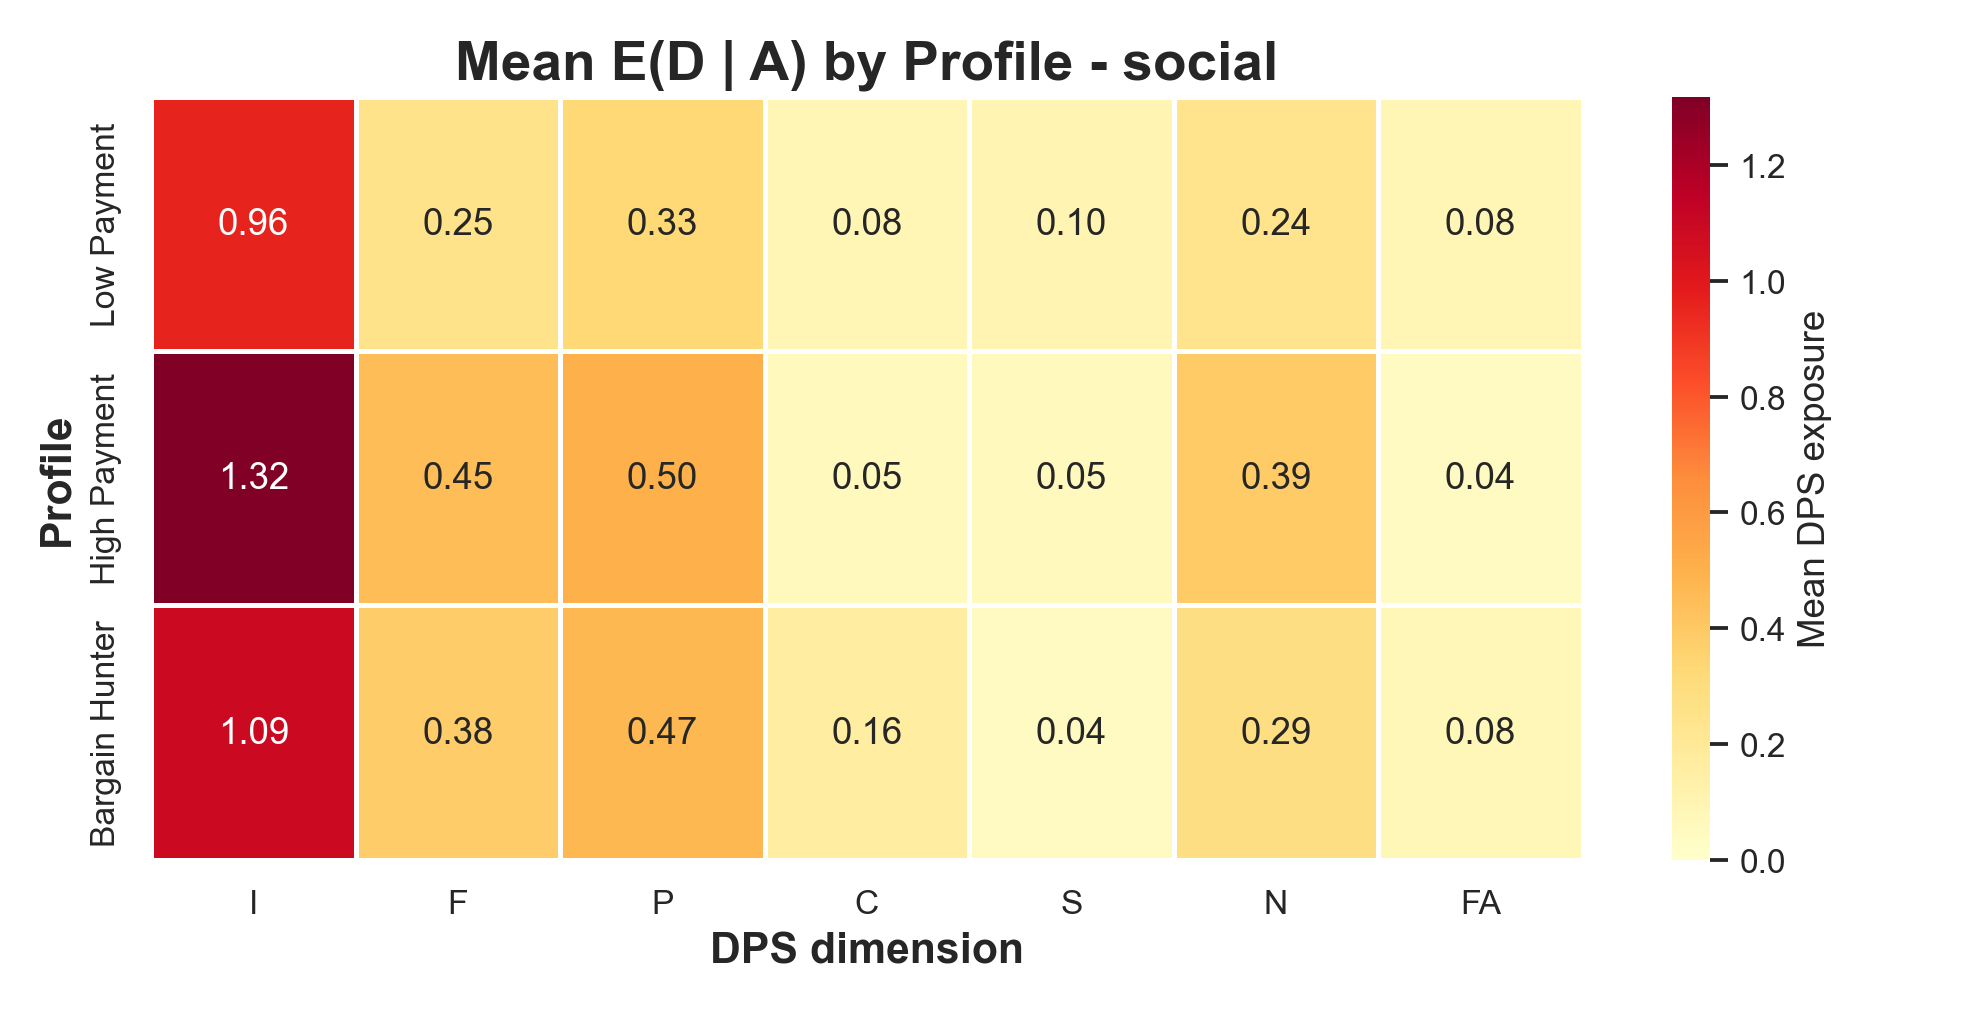
\includegraphics[width=0.95\linewidth]{figures/statistics/heatmap_mean_exposure_social.png}
    \caption{Mean DPS exposure heatmap for social applications.}
    \label{fig:mean-exposure-social}
\end{figure}

\paragraph{Interpretation.}
The profile-level means suggest observed exposure differences rather than a single universal dark-pattern profile for each app, but the averages alone are not sufficiently expressive. The high-payment shopping profile is associated with higher average exposure in Interface Interference and Pressure, which is consistent with trajectories that more often enter purchase, membership, shopping-cart, checkout, or promotion-related interfaces. The bargain-hunter profile also shows relatively high exposure in promotion-sensitive dimensions, which is consistent with searches for discounts, coupons, group-buying opportunities, flash sales, and reward mechanisms. By contrast, the low-payment browsing profile has the lowest aggregate mean, but it still encounters non-trivial Forced Action exposure, such as login, notification, location, or commitment prompts. More importantly, the food-delivery and social results, together with their heatmaps and category-level tables, make the exposure gap visibly clearer: the category-level patterns show a more pronounced separation between profiles than the global averages alone. These results suggest that dark pattern exposure is shaped by the interaction path followed by the user profile, not only by the static presence of interface elements in an app.

\paragraph{Caveat.}
These results should be interpreted as profile-conditioned exposure differences in the observed audit data. The experiment measures visible interface exposure under controlled profiles; it does not reveal the internal decision logic of the applications. Therefore, the findings are best understood as evidence that controlled profiles are associated with different DPS distributions. Whether these differences arise from personalization, rule-based interface flows, recommendation mechanisms, promotion systems, or ordinary navigation differences remains outside the scope of this experiment.

\section{Finding 2: Exposure Estimates Stabilize}

\paragraph{Result.}
The running mean convergence analysis suggests that the exposure estimates become more stable as interaction steps accumulate. Early trajectory segments fluctuate more strongly, while later segments move toward a narrower range. This pattern supports the use of repeated observations rather than isolated screenshots for estimating profile-conditioned exposure.

\paragraph{Evidence.}
For a given profile and DPS dimension, the running mean after step $t$ is calculated from all annotated observations collected from step 1 to step $t$. At the beginning of each exploration trajectory, a single pop-up, login prompt, checkout page, or promotional banner can strongly affect the cumulative average because the sample size is still small. After repeated interactions, the curves gradually become smoother. Most dimensions stabilize within the 20--30 step range used by the audit protocol, which indicates that the final profile-level estimates are less sensitive to any single screen state.

\paragraph{WangYiYun example.}
The WangYiYun trajectories provide a concrete illustration of this stabilization pattern at the single-application level. Figures~\ref{fig:wangyiyun-curve-high}, \ref{fig:wangyiyun-curve-low}, and \ref{fig:wangyiyun-curve-bargain} show the running mean exposure curves for the high-payment shopping, low-payment browsing, and bargain-hunter profiles, respectively. Although the early steps fluctuate more strongly, the later segments become visibly smoother, especially for the dominant dimensions that remain active across repeated interactions.

\begin{figure}[htbp]
    \centering
    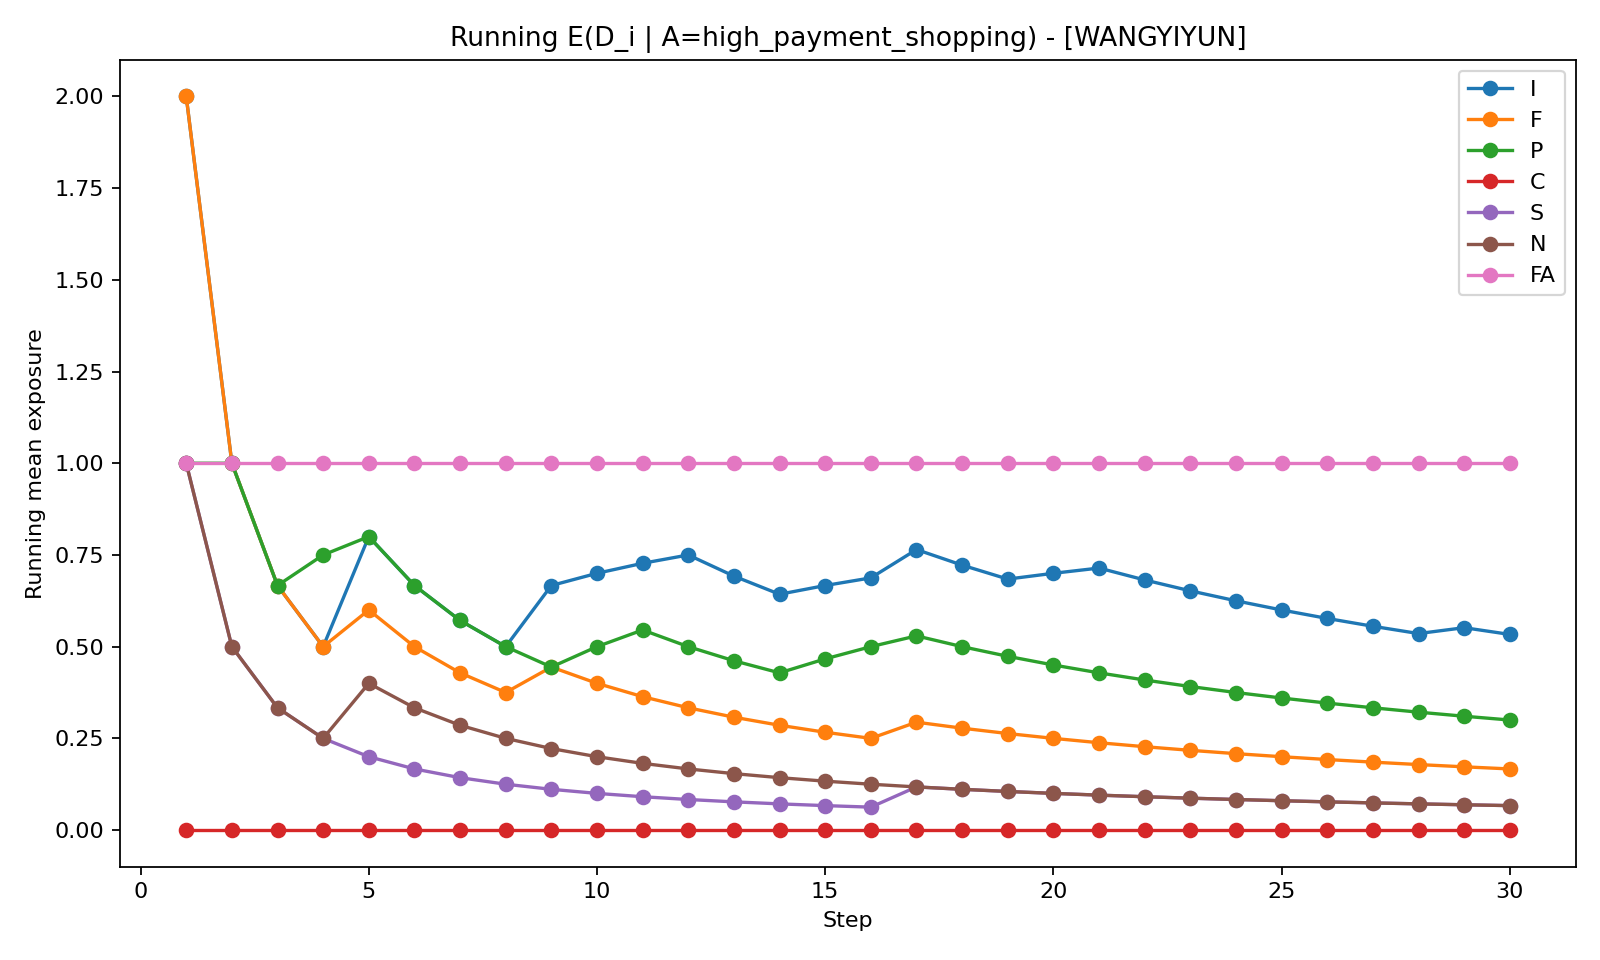
\includegraphics[width=0.85\linewidth]{figures/statistics/curves_entertainment/curve_E_high_payment_shopping_WangYiYun_entertainment.png}
    \caption{Running mean DPS exposure curve for WangYiYun under the high-payment shopping profile.}
    \label{fig:wangyiyun-curve-high}
\end{figure}

\begin{figure}[htbp]
    \centering
    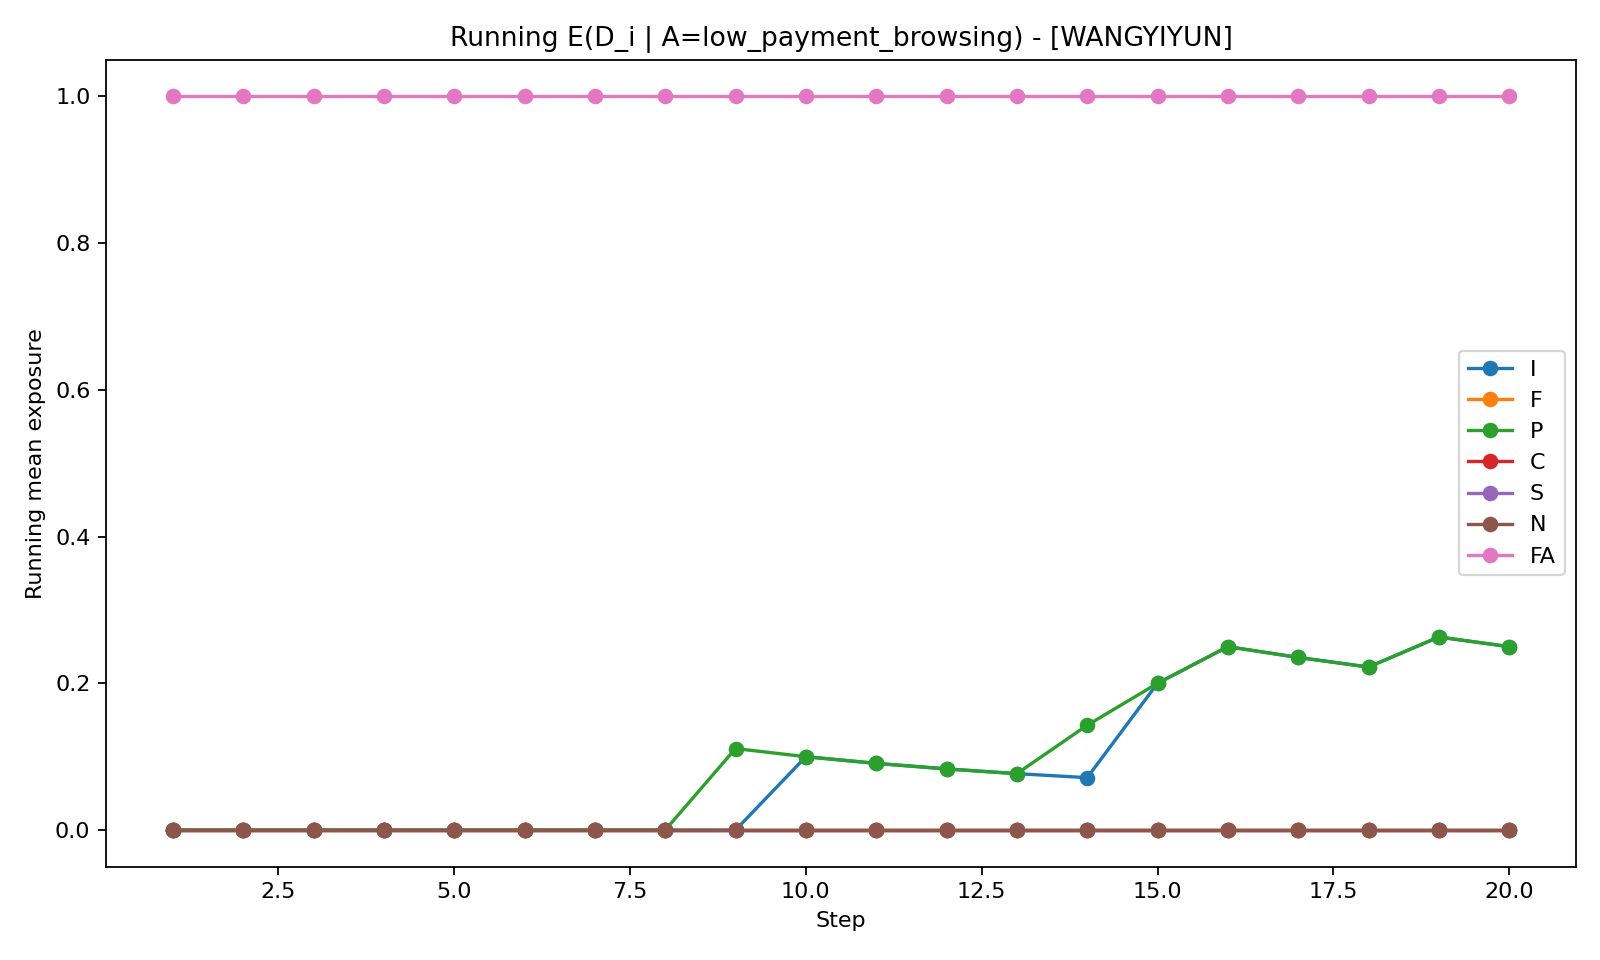
\includegraphics[width=0.85\linewidth]{figures/statistics/curves_entertainment/curve_E_low_payment_browsing_WangYiYun_entertainment.png}
    \caption{Running mean DPS exposure curve for WangYiYun under the low-payment browsing profile.}
    \label{fig:wangyiyun-curve-low}
\end{figure}

\begin{figure}[htbp]
    \centering
    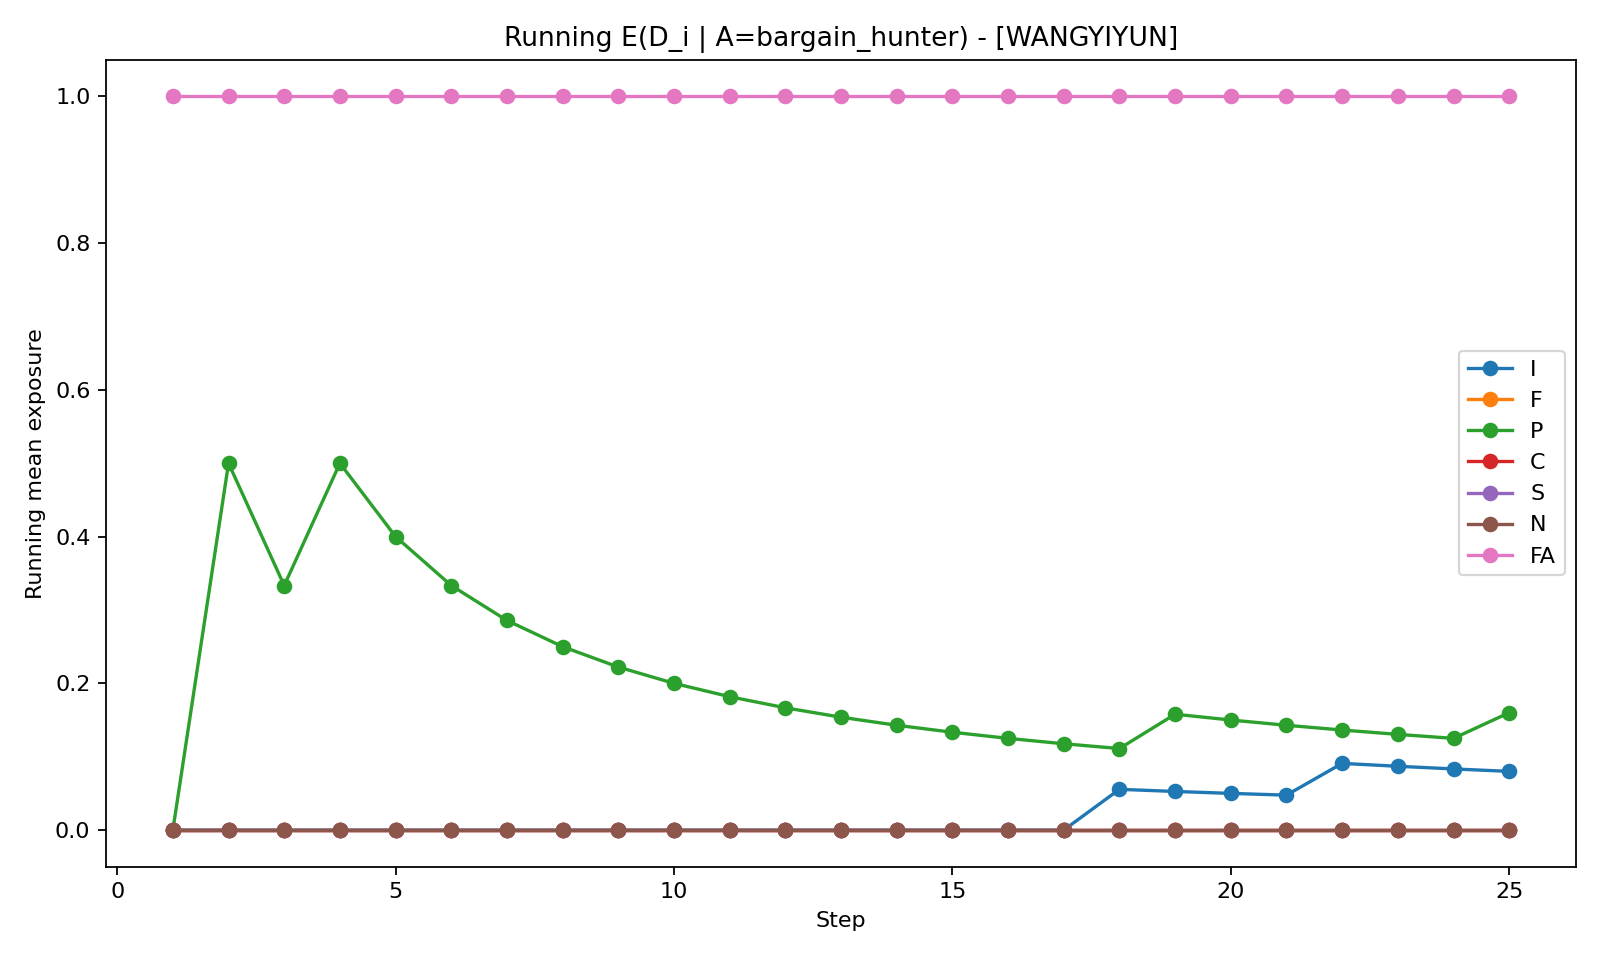
\includegraphics[width=0.85\linewidth]{figures/statistics/curves_entertainment/curve_E_bargain_hunter_WangYiYun_entertainment.png}
    \caption{Running mean DPS exposure curve for WangYiYun under the bargain-hunter profile.}
    \label{fig:wangyiyun-curve-bargain}
\end{figure}

\paragraph{Interpretation.}
The convergence pattern supports the methodological choice of treating exposure as an expectation, denoted as $E(D \mid A)$, rather than as a simple count of detected dark pattern instances. A count-based measure can show how many times a label appears, but it does not directly express the average exposure level associated with a profile-conditioned trajectory. The running mean curves make this expectation-based interpretation visible. As the trajectory grows longer, the estimate becomes less sensitive to individual screens and more representative of the profile's typical exposure pattern in that app or category. This design follows the broader logic of algorithm auditing and exposure measurement, where repeated observations are needed to characterize the behavior of black-box systems under controlled conditions \cite{sandvig2014auditing,hannak2013personalization,srba2023youtube}.

\paragraph{Caveat.}
Stabilization within the audited trajectories does not mean that all possible dark pattern exposure in an application has been exhausted. Some dark patterns may appear only after longer-term use, repeated purchases, account aging, seasonal promotions, or accumulated behavioral history. In addition, the archived result files show that a small number of app-profile runs contain fewer than the planned 30 steps. The convergence result therefore supports the reliability of this course-scale experiment, but it does not remove the need for longer-term or larger-scale audits.

\section{Finding 3: Statistical Evidence for Profile-dependent Exposure}

\begin{figure}[htbp]
    \centering
    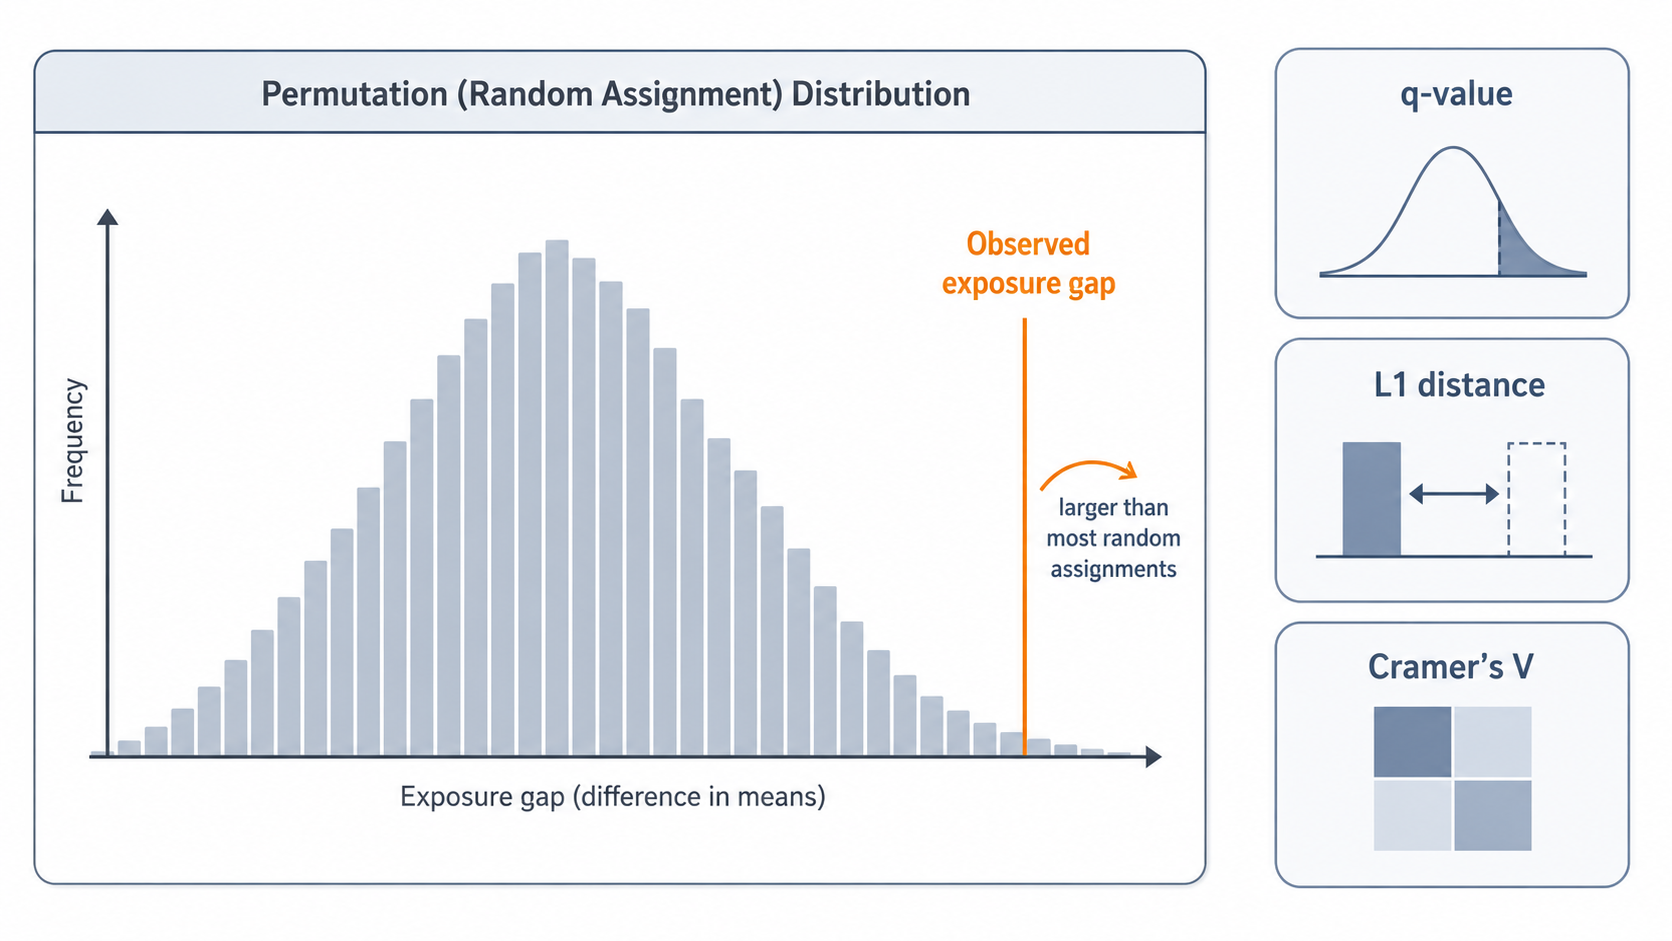
\includegraphics[width=0.95\linewidth]{figures/pictures/permutation_test_intuition.png}
    \caption{Permutation Test Intuition}
    \label{fig:permutation_test_intuition}
\end{figure}

\paragraph{Result.}
The statistical tests provide mixed but informative evidence for profile-dependent exposure. Across all apps, the low-payment browsing and high-payment shopping profiles differ significantly after false-discovery-rate correction. At the category level, the strongest evidence appears in eating and social applications, while the entertainment category does not show statistically robust pairwise differences under the permutation tests.

\begin{table}[htbp]
    \centering
    \caption{Statistical summary of profile-dependent DPS exposure differences.}
    \label{tab:statistical-summary}
    \footnotesize
    \setlength{\tabcolsep}{4pt}
    \renewcommand{\arraystretch}{1.08}
    \begin{tabular}{@{}p{0.26\linewidth}p{0.09\linewidth}p{0.08\linewidth}p{0.08\linewidth}p{0.08\linewidth}p{0.08\linewidth}p{0.28\linewidth}@{}}
        \toprule
        Comparison & Scope & $p$-value & $q$-value & L1 distance & Cramér's $V$ & Interpretation \\
        \midrule
        Low browsing vs. High shopping & All & 0.0082 & 0.0246 & 0.301 & 0.050 & FDR-significant difference \\
        Low browsing vs. Bargain hunter & All & 0.0832 & 0.1248 & 0.227 & 0.078 & Not statistically robust \\
        High shopping vs. Bargain hunter & All & 0.3633 & 0.3633 & 0.164 & 0.061 & Not statistically robust \\
        Low browsing vs. High shopping & Eating & 0.0018 & 0.0054 & 0.542 & 0.129 & FDR-significant difference \\
        Low browsing vs. Bargain hunter & Eating & 0.0072 & 0.0108 & 0.467 & 0.155 & FDR-significant difference \\
        High shopping vs. Bargain hunter & Eating & 0.1776 & 0.1776 & 0.292 & 0.134 & Not statistically robust \\
        Low browsing vs. High shopping & Entertainment & 0.8386 & 0.8644 & 0.187 & 0.159 & Not statistically robust \\
        Low browsing vs. Bargain hunter & Entertainment & 0.5505 & 0.8644 & 0.269 & 0.156 & Not statistically robust \\
        High shopping vs. Bargain hunter & Entertainment & 0.8644 & 0.8644 & 0.186 & 0.047 & Not statistically robust \\
        Low browsing vs. High shopping & Shopping & 0.0784 & 0.1176 & 0.200 & 0.100 & Not statistically robust \\
        Low browsing vs. Bargain hunter & Shopping & 0.2759 & 0.2759 & 0.175 & 0.113 & Not statistically robust \\
        High shopping vs. Bargain hunter & Shopping & 0.0058 & 0.0174 & 0.325 & 0.180 & FDR-significant difference \\
        Low browsing vs. High shopping & Social & 0.0002 & 0.0006 & 0.997 & 0.155 & FDR-significant difference \\
        Low browsing vs. Bargain hunter & Social & 0.0400 & 0.0400 & 0.585 & 0.125 & FDR-significant difference \\
        High shopping vs. Bargain hunter & Social & 0.0388 & 0.0400 & 0.584 & 0.149 & FDR-significant difference \\
        \bottomrule
    \end{tabular}
\end{table}

\paragraph{Evidence.}
Figures~\ref{fig:mannwhitney-qvalue-all}, \ref{fig:permutation-pvalues}, \ref{fig:permutation-l1}, and \ref{fig:cramers-v} report the statistical validation results used to evaluate profile-dependent exposure differences. Table~\ref{tab:statistical-summary} summarizes the numerical results from the repository's statistical-test CSV files. The first figure is a dimension-level Mann-Whitney U BH FDR q-value heatmap, whereas the permutation figures summarize profile-label randomization at the profile-comparison scope. The permutation tests evaluate whether observed exposure gaps are larger than what would be expected under random profile assignment. The q-values adjust significance interpretation across multiple comparisons using Benjamini-Hochberg FDR correction. The L1 distance measures the practical magnitude of differences between DPS exposure vectors. Cramér's V measures the association strength between profile type and DPS exposure.

\begin{figure}[htbp]
    \centering
    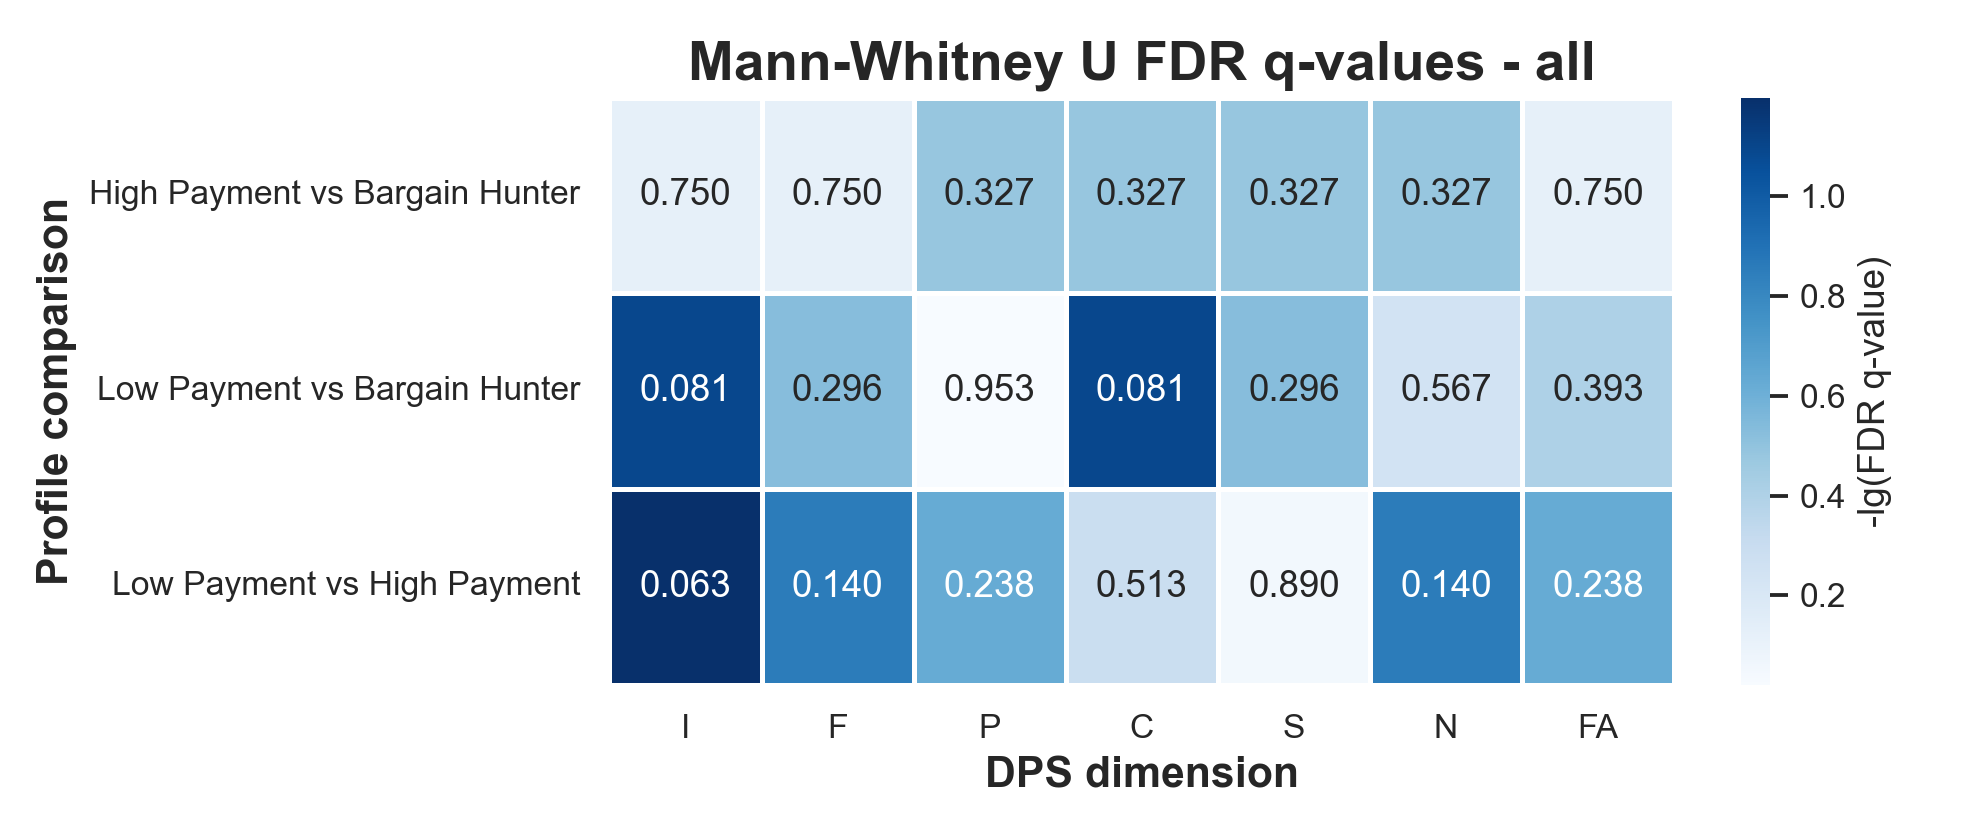
\includegraphics[width=0.95\linewidth]{figures/statistics/mannwhitney_qvalue_heatmap_all.png}
    \caption{Mann-Whitney U BH FDR q-value heatmap for dimension-level DPS exposure comparisons across all audited applications.}
    \label{fig:mannwhitney-qvalue-all}
\end{figure}

\begin{figure}[htbp]
    \centering
    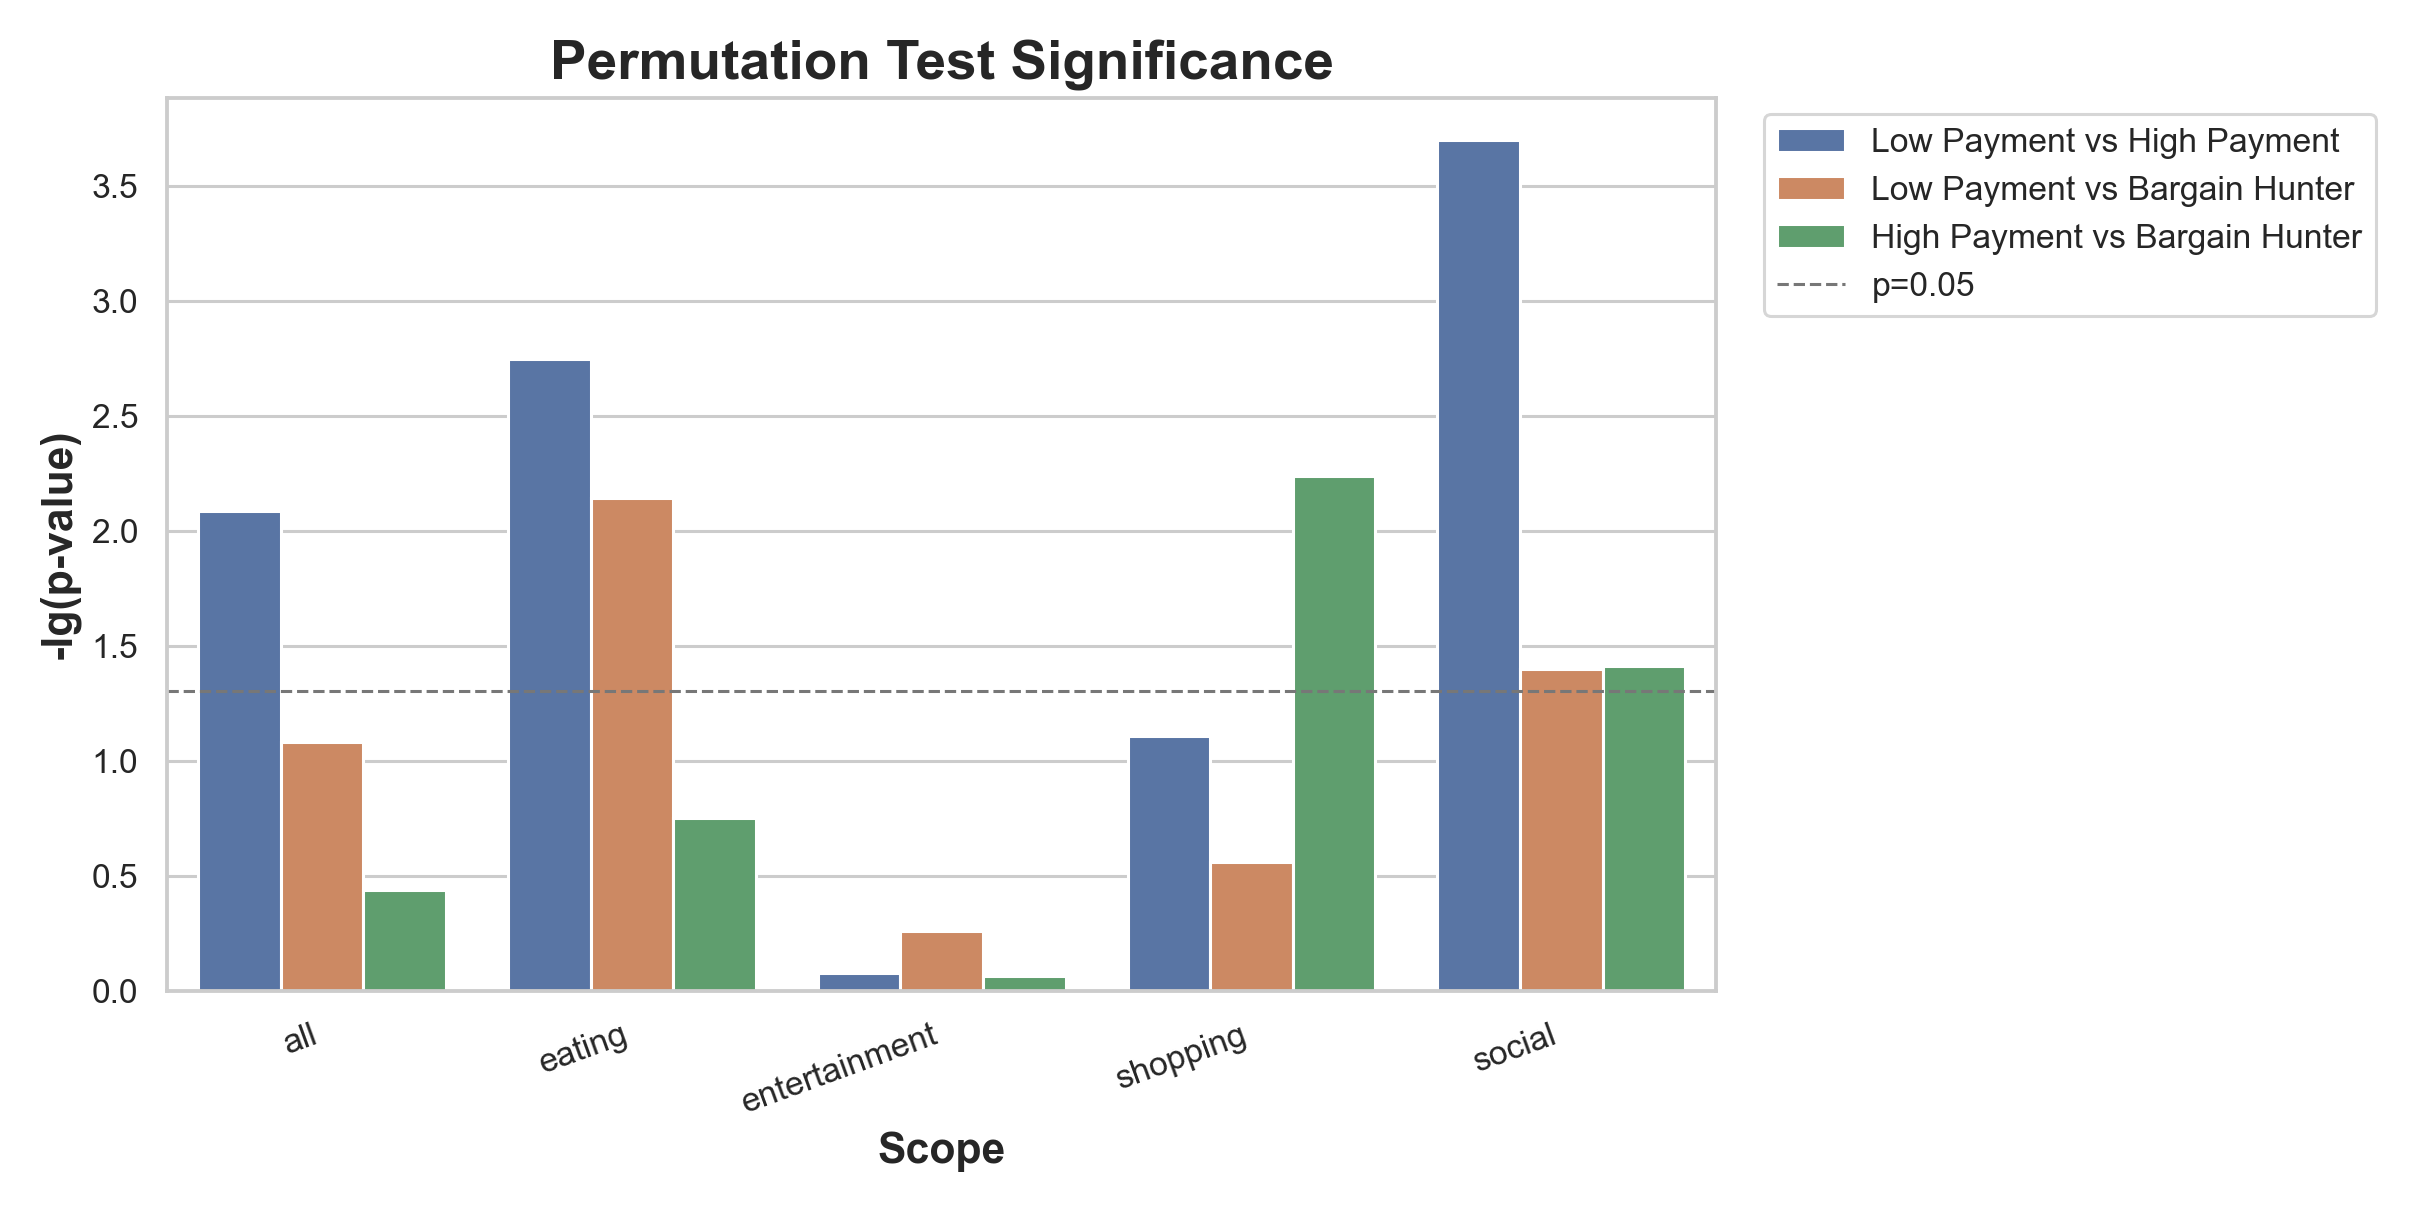
\includegraphics[width=0.95\linewidth]{figures/statistics/permutation_pvalues_by_scope.png}
    \caption{Permutation-test p-values by comparison scope.}
    \label{fig:permutation-pvalues}
\end{figure}

\begin{figure}[htbp]
    \centering
    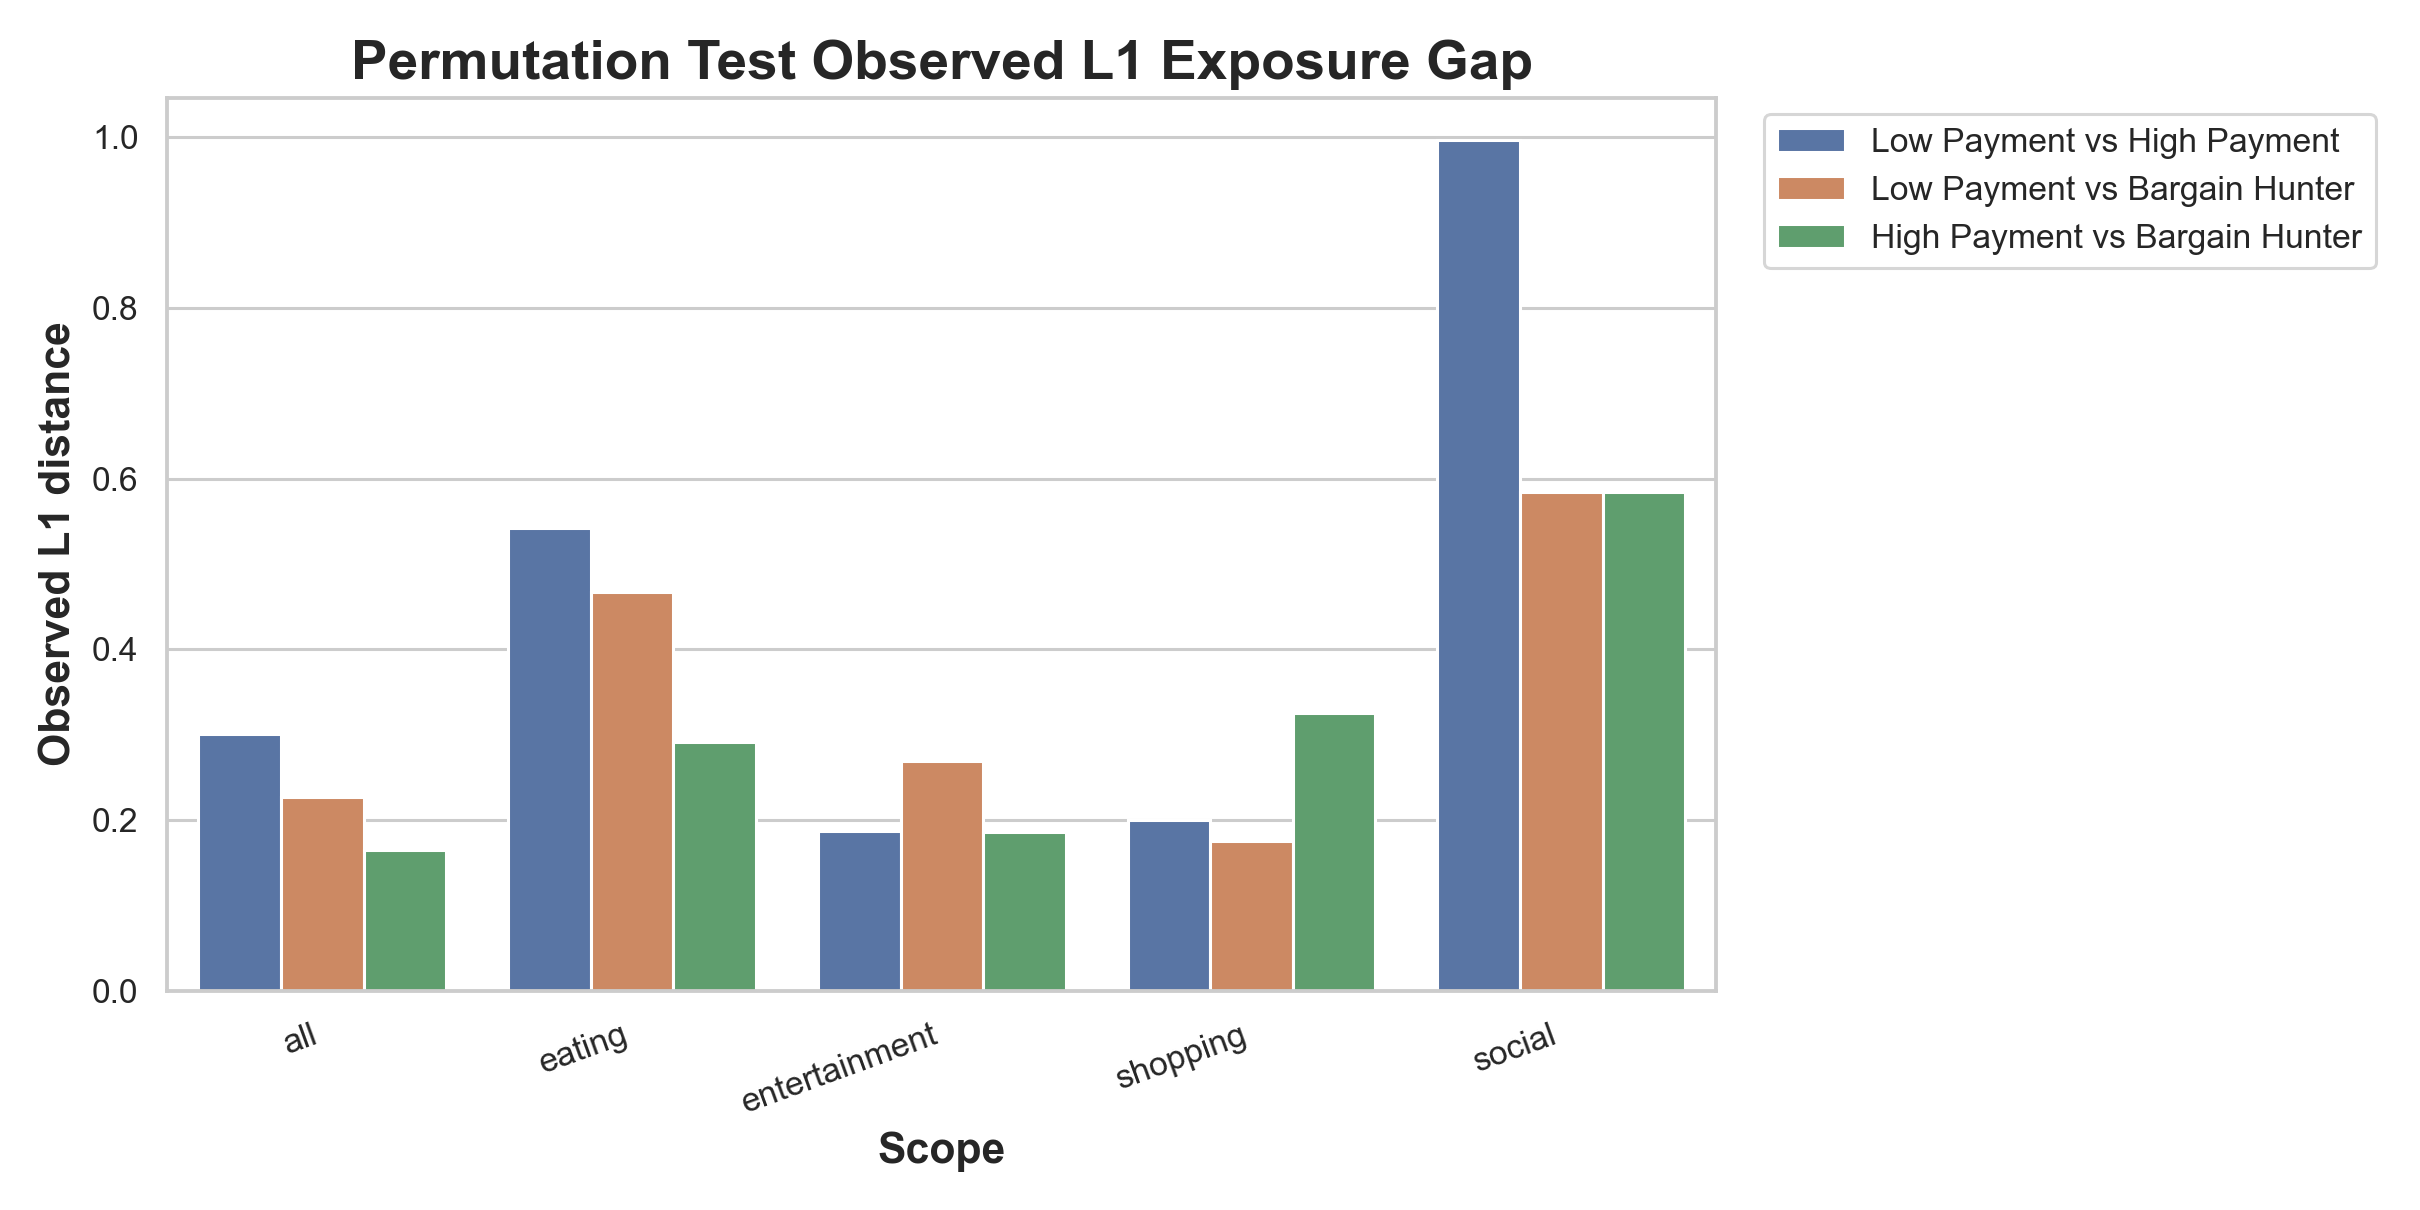
\includegraphics[width=0.95\linewidth]{figures/statistics/permutation_observed_l1_by_scope.png}
    \caption{Observed L1 exposure distances by comparison scope.}
    \label{fig:permutation-l1}
\end{figure}

\begin{figure}[htbp]
    \centering
    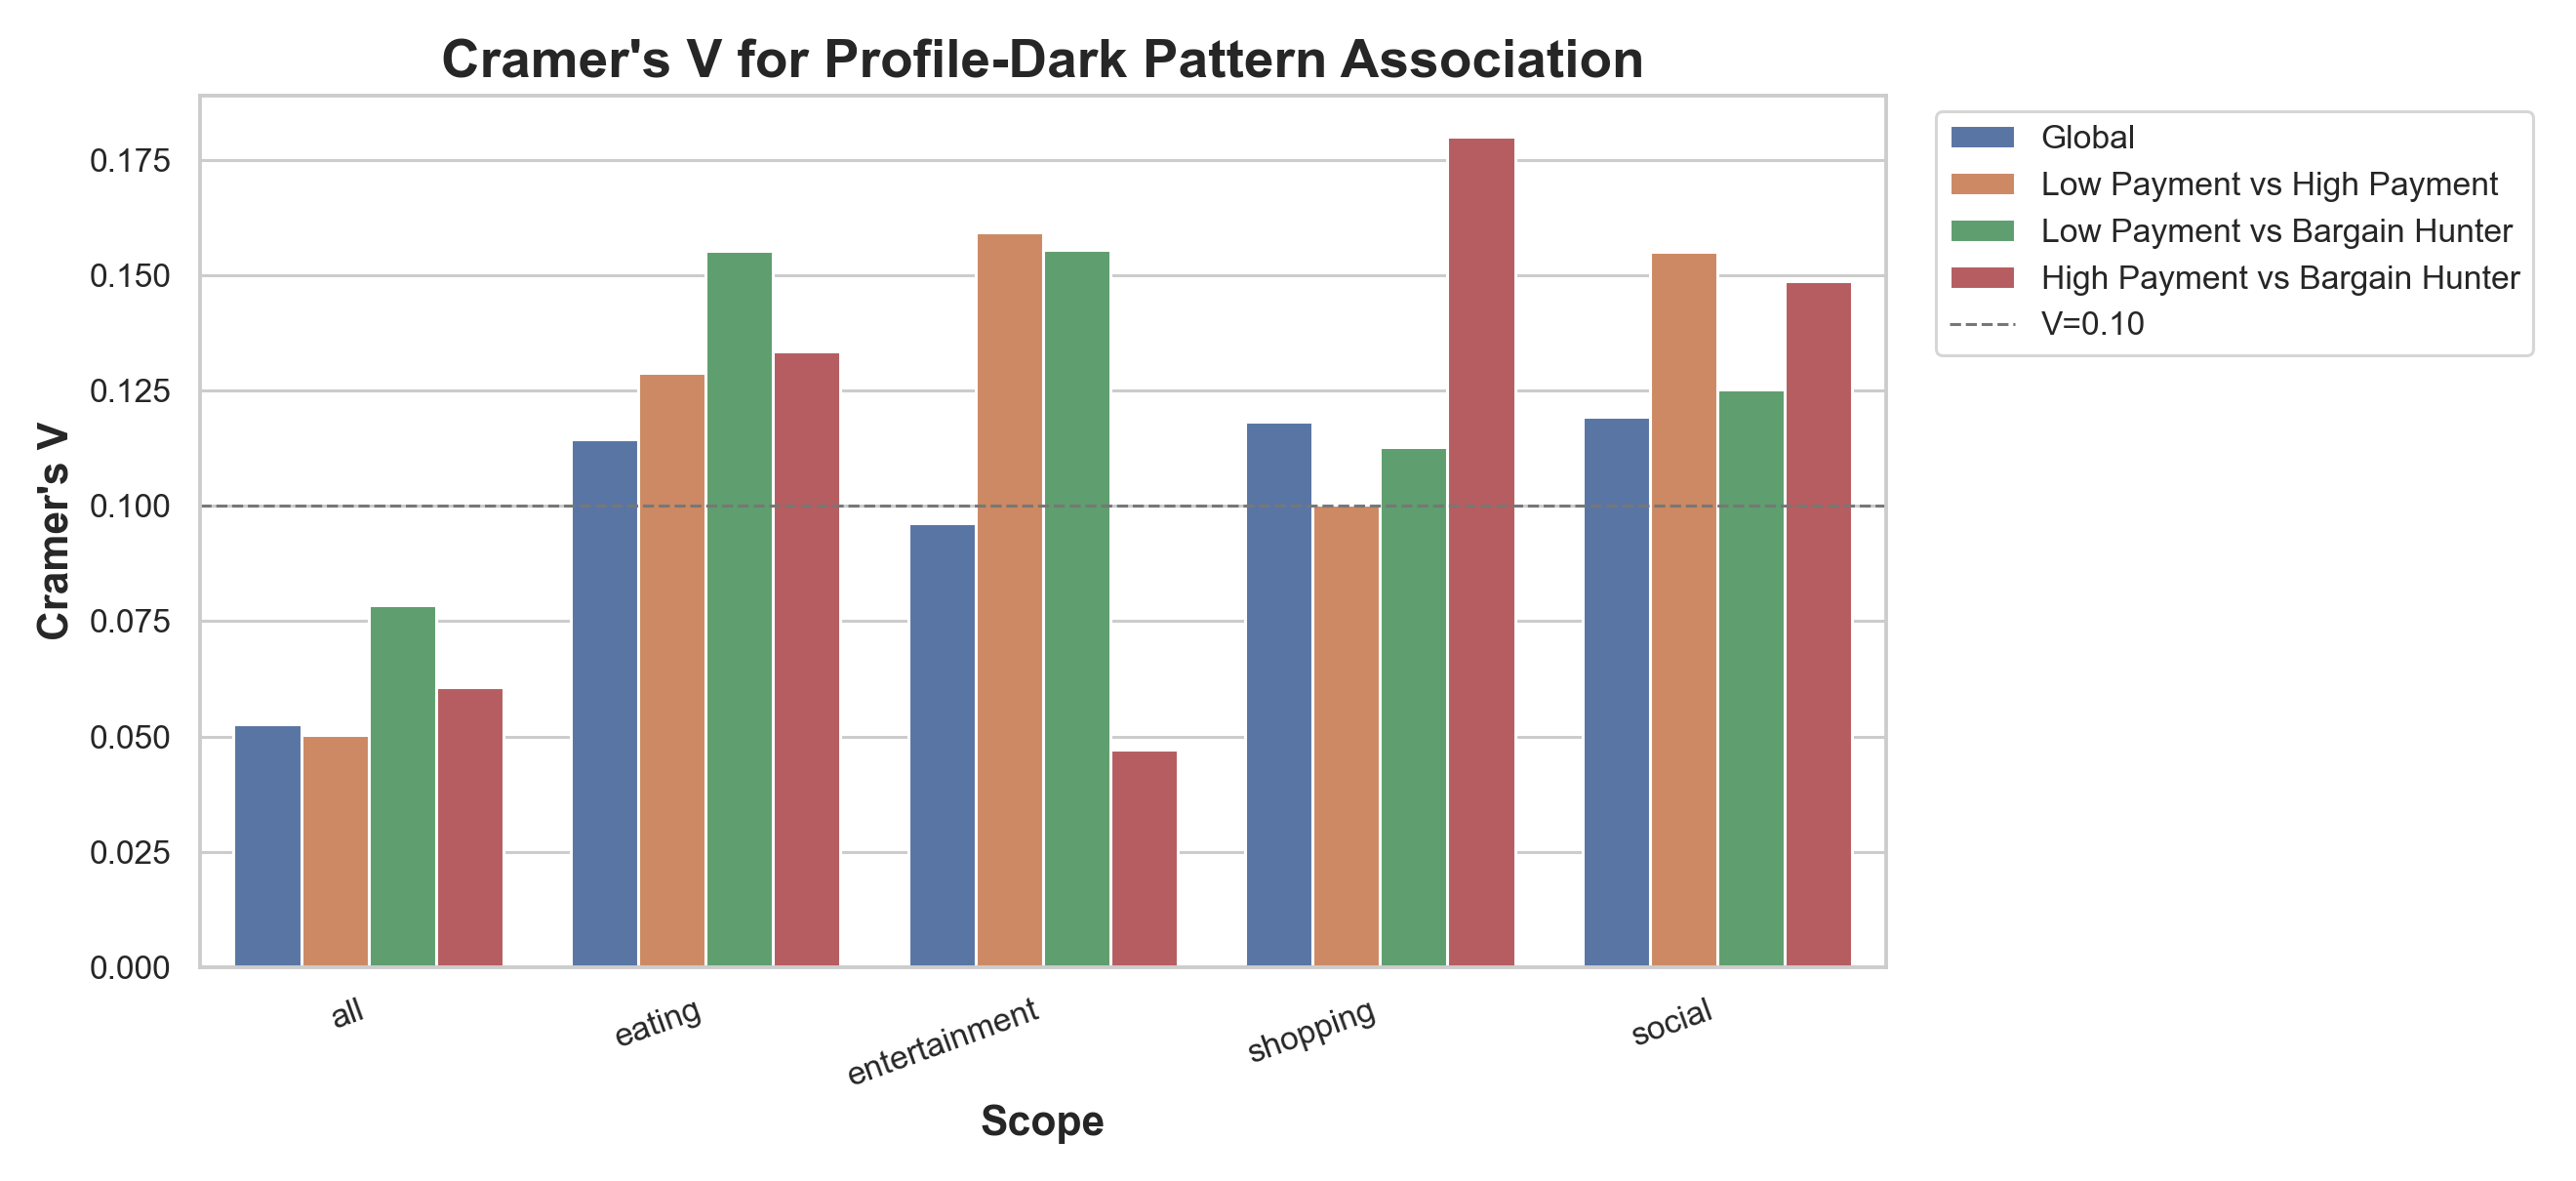
\includegraphics[width=0.95\linewidth]{figures/statistics/cramers_v_by_scope.png}
    \caption{Cramér's \(V\) association strength by comparison scope.}
    \label{fig:cramers-v}
\end{figure}

\paragraph{Interpretation.}
The all-app comparison suggests that low-payment browsing and high-payment shopping are associated with different exposure distributions. The category-level results further show that observed exposure differences are not evenly distributed across app domains. Eating and social applications show several FDR-significant pairwise comparisons, and shopping applications show a significant difference between high-payment shopping and bargain-hunter profiles. Entertainment applications, by contrast, do not show statistically robust pairwise differences in the current result files. The L1 distances help distinguish practical exposure gaps from purely statistical effects, while Cramér's V indicates that the observed associations are generally small to modest.

\paragraph{Caveat.}
The statistical evidence should be interpreted as association, not as evidence about internal app mechanisms. The permutation tests depend on the observed audit sample, the q-values depend on the chosen family of comparisons, and Cramér's V is computed from binary contingency summaries built from DPS presence versus absence. These metrics therefore strengthen the claim that observed exposure differences exist in the audited data, but they do not identify whether those differences come from personalization, recommendation flows, promotion modules, permissions, login gates, or ordinary navigation paths.

\section{Category-level Observations}

Beyond profile-level differences, the results also reveal several category-level patterns. These observations should be interpreted as empirical patterns from the audited applications and as plausible interpretations of interface mechanisms, rather than universal claims about all applications in a category. Figures~\ref{fig:category-heatmap-shopping}, \ref{fig:category-heatmap-eating}, \ref{fig:category-heatmap-entertainment}, and \ref{fig:category-heatmap-social} summarize category-level exposure patterns.

\begin{figure}[htbp]
    \centering
    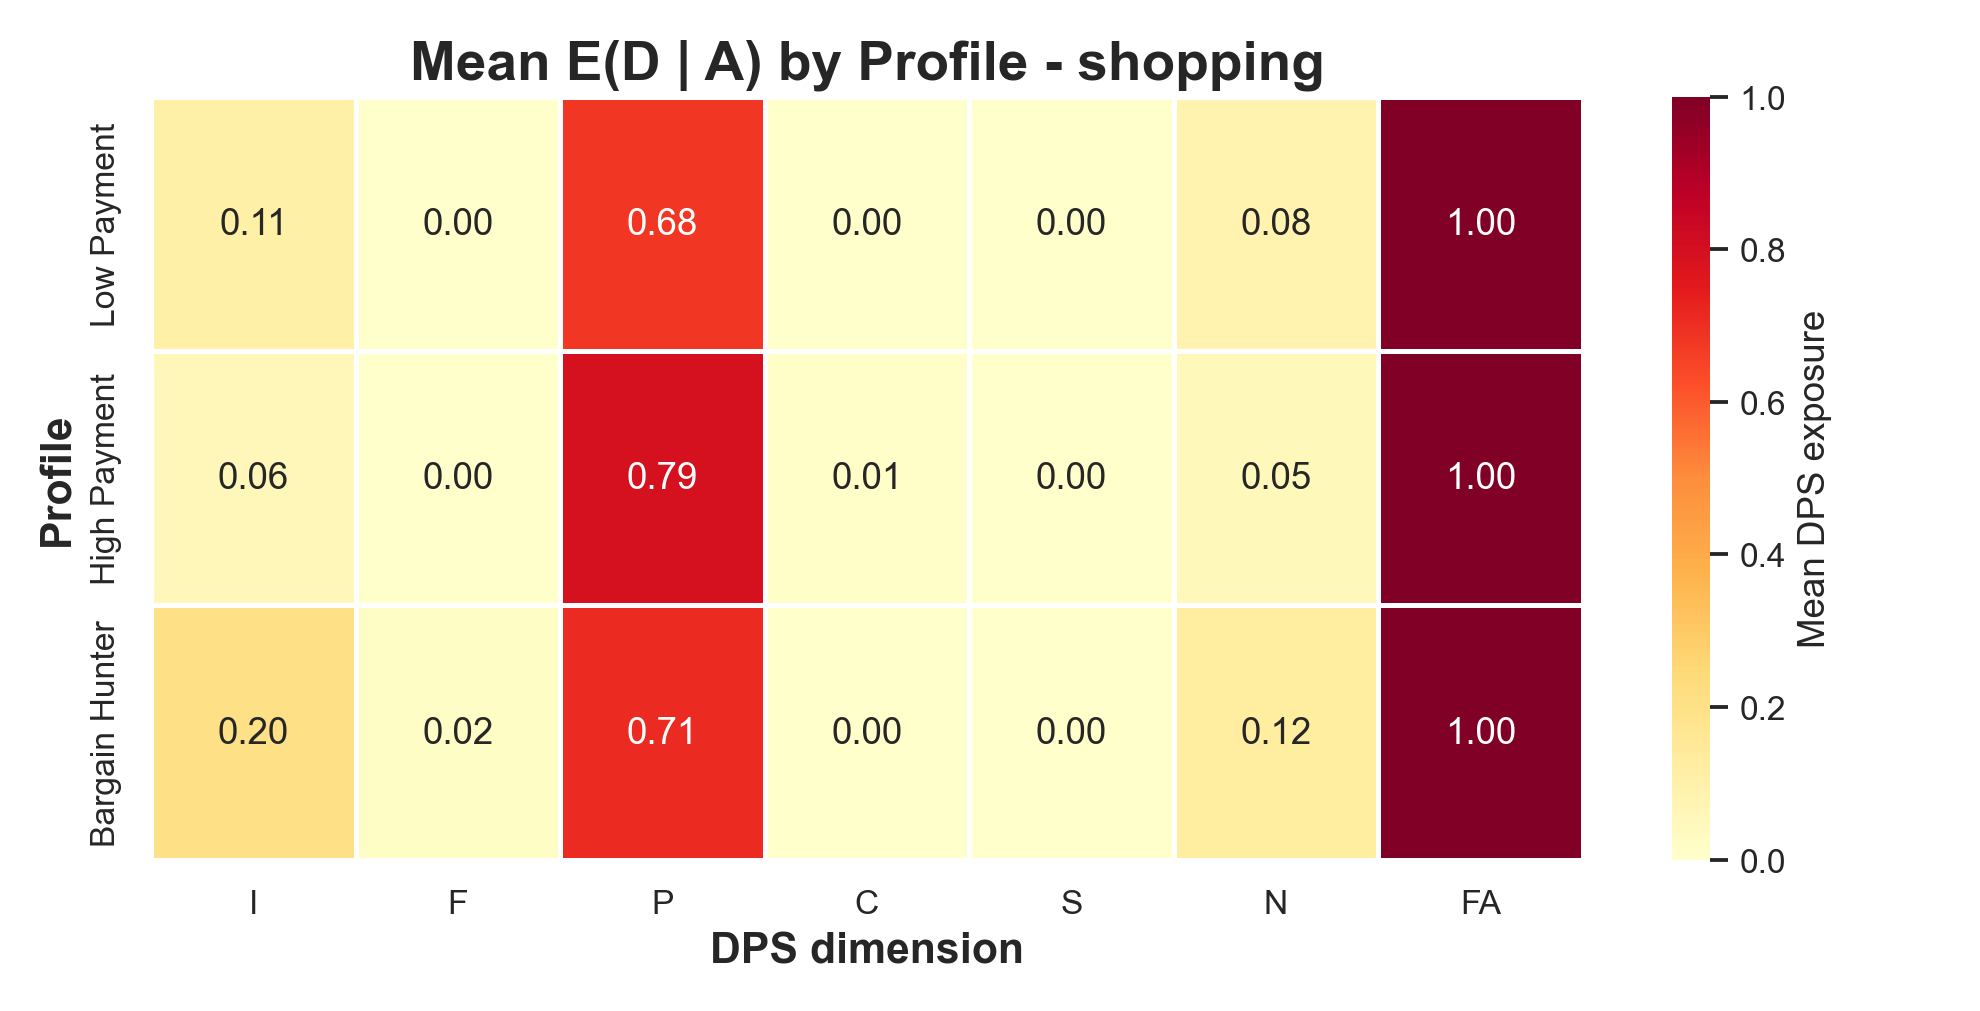
\includegraphics[width=0.95\linewidth]{figures/statistics/heatmap_mean_exposure_shopping.png}
    \caption{Mean DPS exposure heatmap for shopping applications.}
    \label{fig:category-heatmap-shopping}
\end{figure}

\begin{figure}[htbp]
    \centering
    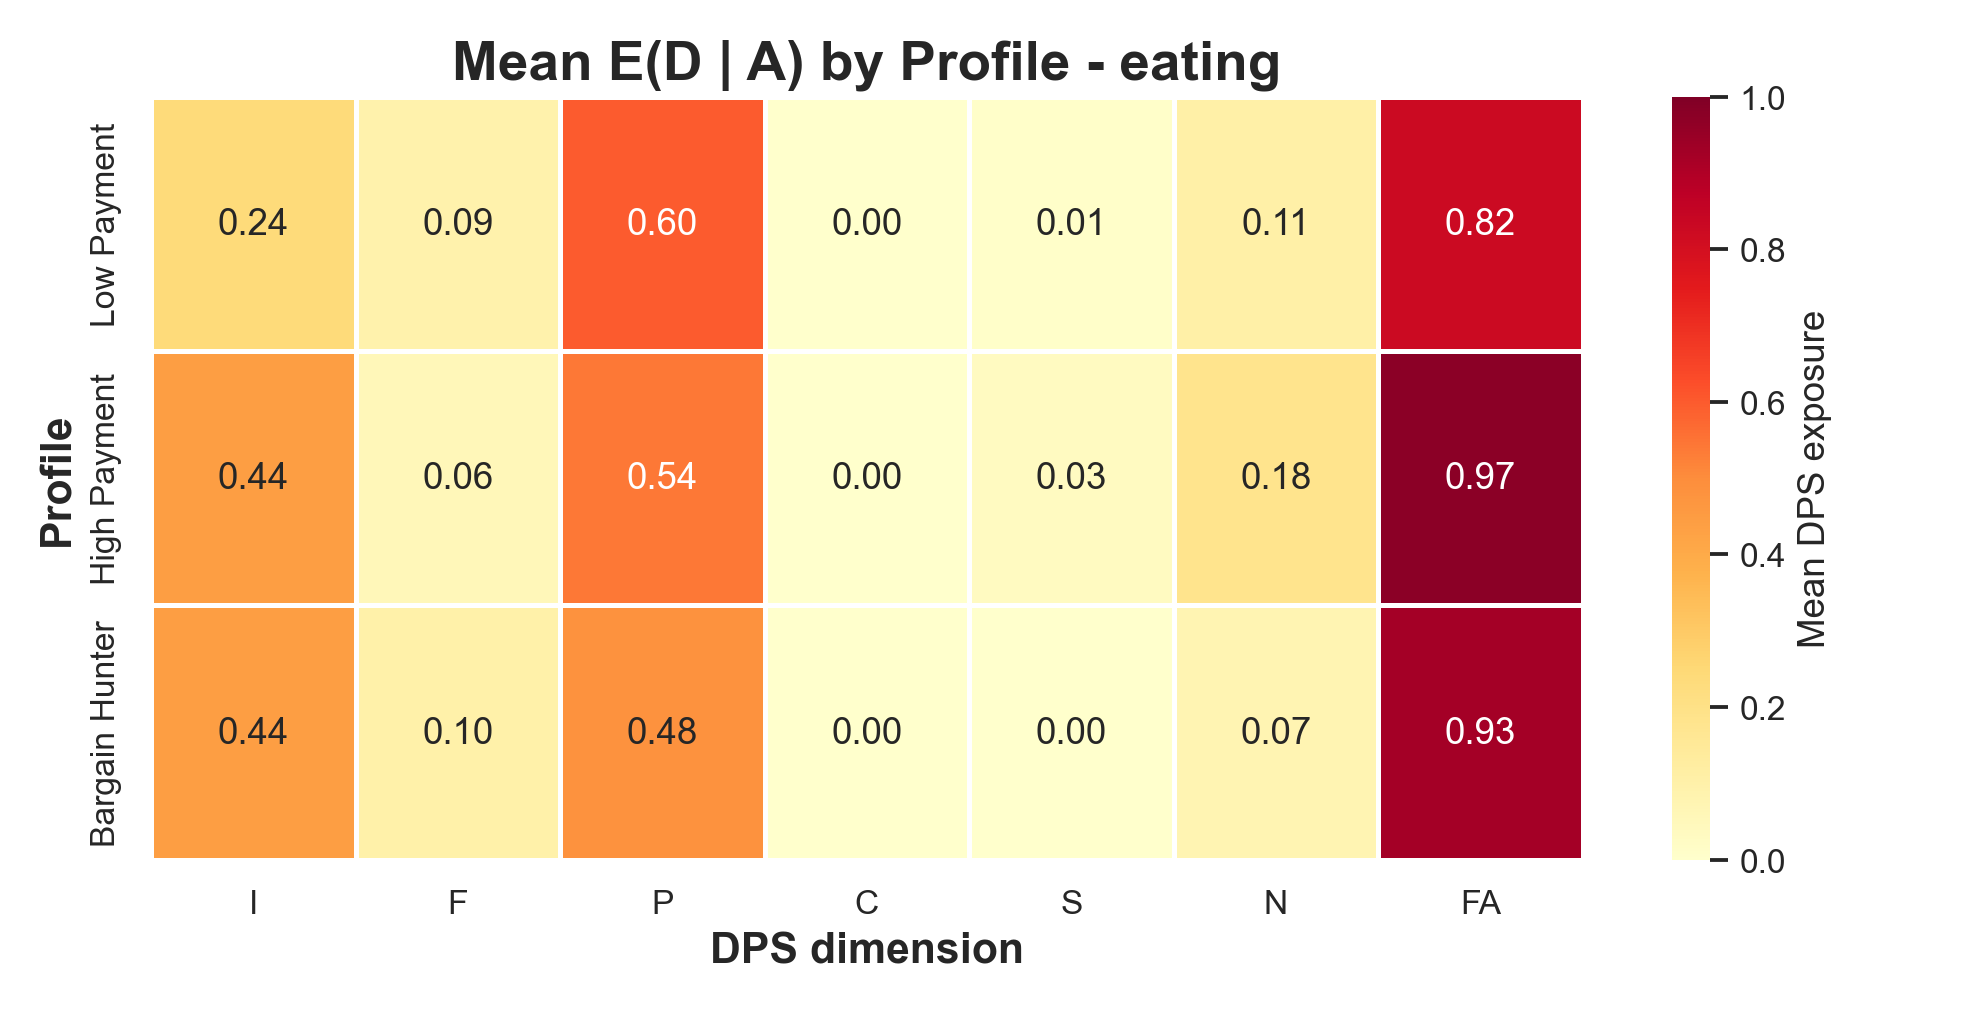
\includegraphics[width=0.95\linewidth]{figures/statistics/heatmap_mean_exposure_eating.png}
    \caption{Mean DPS exposure heatmap for food-delivery and eating-related applications.}
    \label{fig:category-heatmap-eating}
\end{figure}

\begin{figure}[htbp]
    \centering
    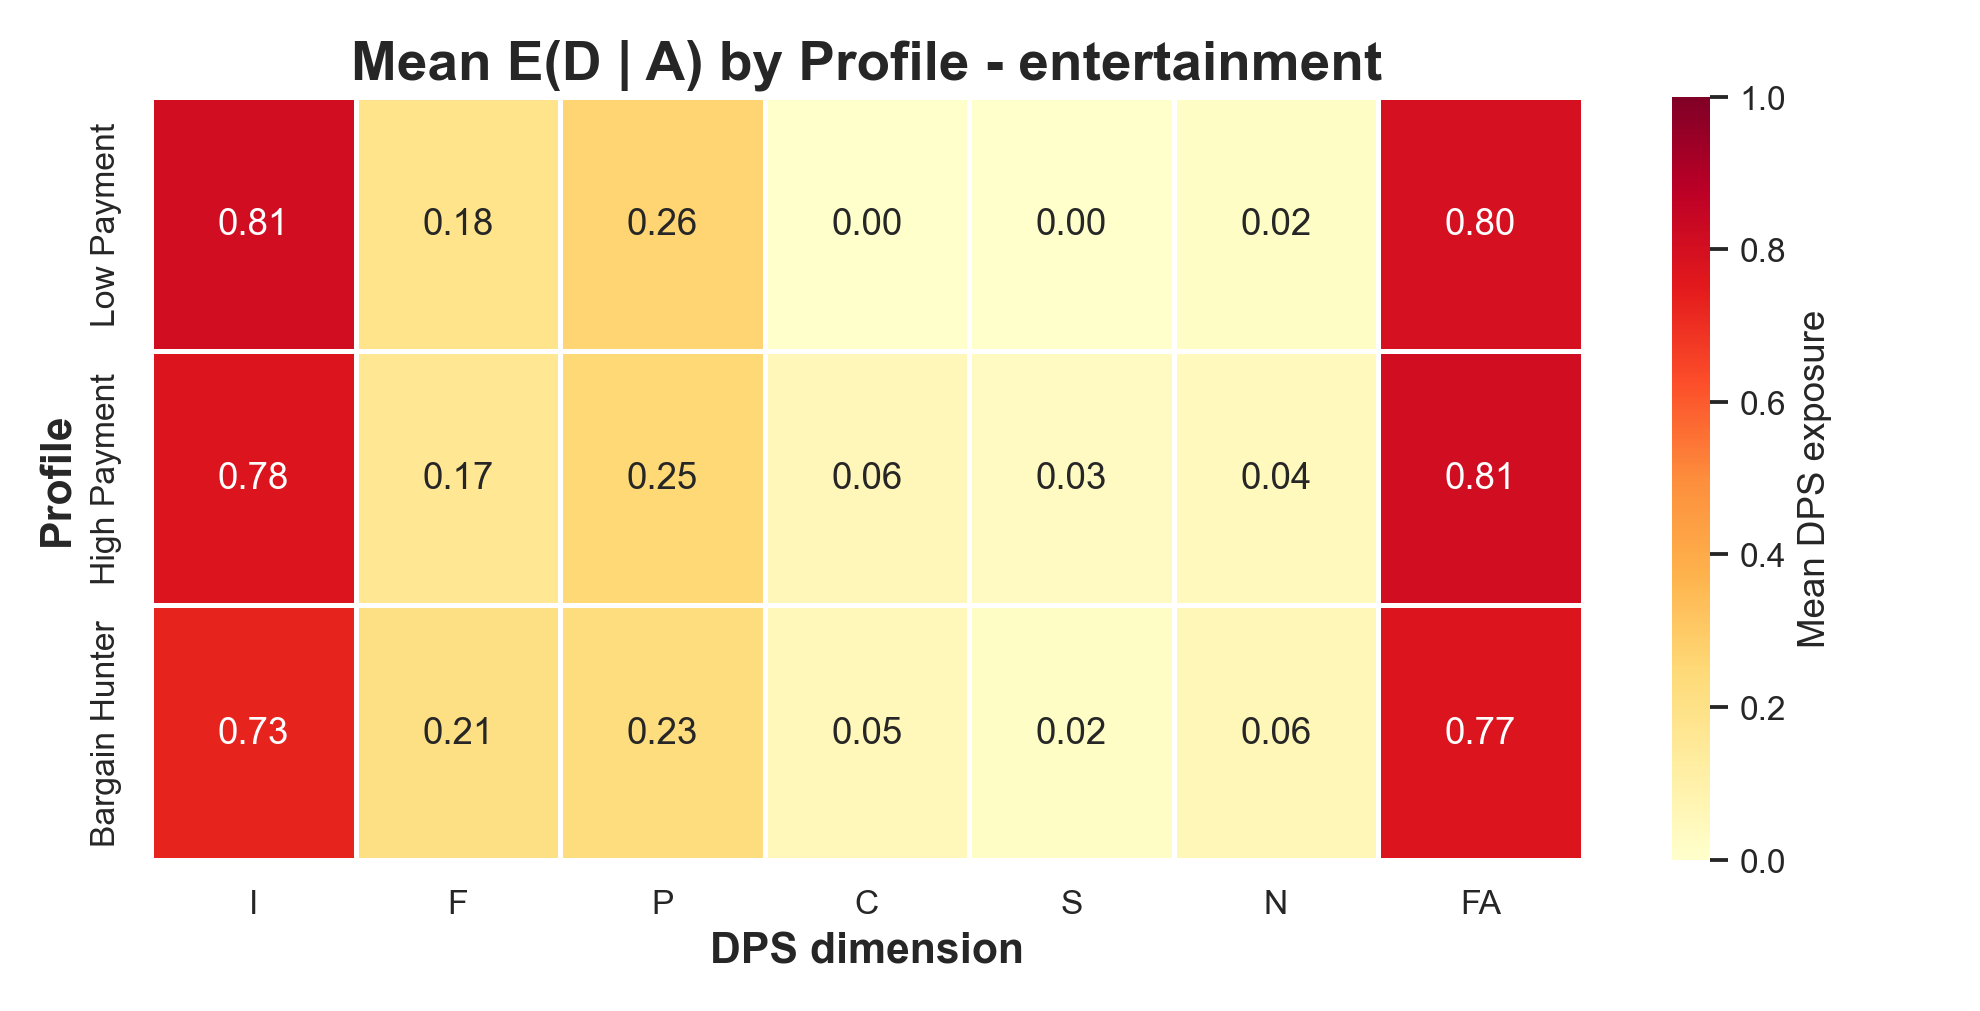
\includegraphics[width=0.95\linewidth]{figures/statistics/heatmap_mean_exposure_entertainment.png}
    \caption{Mean DPS exposure heatmap for entertainment applications.}
    \label{fig:category-heatmap-entertainment}
\end{figure}

\begin{figure}[htbp]
    \centering
    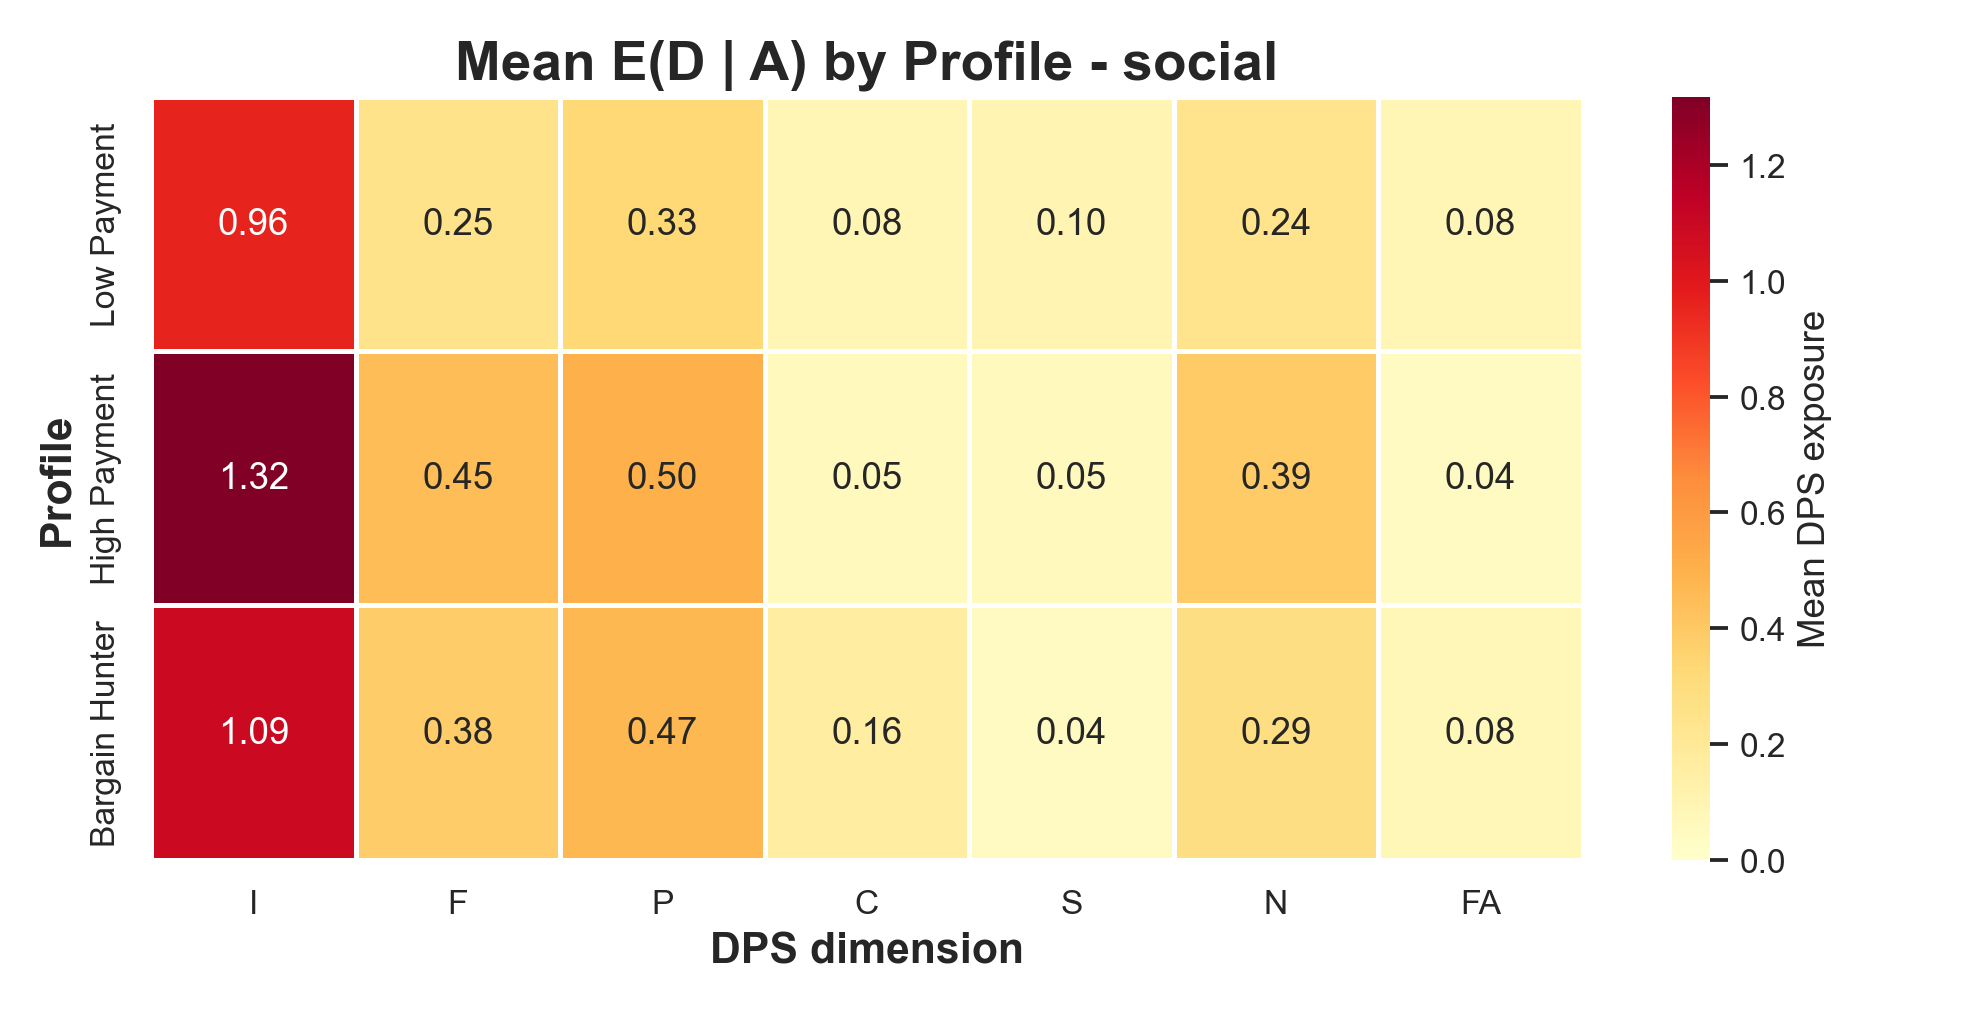
\includegraphics[width=0.95\linewidth]{figures/statistics/heatmap_mean_exposure_social.png}
    \caption{Mean DPS exposure heatmap for social applications.}
    \label{fig:category-heatmap-social}
\end{figure}

For e-commerce applications, the most prominent dimensions are Pressure, Sneaking, and Interface Interference. This pattern is consistent with the commercial structure of shopping interfaces. Users are frequently guided through product recommendation pages, discount panels, membership prompts, shopping carts, and checkout-related screens. In these contexts, applications may emphasize limited-time discounts, visually prioritize promotional options, preselect certain benefits, or make alternative choices less visible. The high-payment and bargain-hunter profiles are especially likely to encounter such interfaces because their keyword and action distributions lead them toward commercial decision points. These observations align with prior studies showing that shopping environments are common sites for scarcity messages, social proof, hidden costs, and other manipulative design strategies \cite{mathur2019darkpatterns}.

Food-delivery applications show consistently high Forced Action exposure in the project results. This may be associated with interface flows that require location access, login, phone verification, address selection, or permission granting before users can fully browse menus, place orders, or access coupons. Pressure and Nagging also appear in this category, often through repeated prompts for membership, coupons, delivery discounts, push notifications, or limited-time offers. Because food-delivery apps often combine urgent consumption contexts with location-based services and promotional systems, users may encounter multiple forms of commitment-requesting interfaces. However, this should be understood as an observed pattern in the audited sample rather than a universal property of all food-delivery applications.

Content platforms show a different exposure profile. Instead of checkout-oriented pressure, they more frequently involve login prompts, notification prompts, recommendation loops, and nagging. A user may be repeatedly encouraged to sign in, enable notifications, follow accounts, remain in the feed, or continue consuming recommended content. These mechanisms may not always correspond to direct commercial payment, but they can still shape user autonomy and attention. For example, recommendation loops may keep users in a sequence of suggested content, while notification prompts may repeatedly interrupt browsing. Such patterns suggest that dark pattern exposure in content platforms is often related to engagement retention rather than immediate purchase conversion.

Lifestyle service applications show more mixed patterns, including Contextual Deception, Friction, and promotional Pressure. These applications may include booking flows, service reservations, membership benefits, location-based recommendations, and promotional bundles. Contextual deception may appear when an interface leads users to expect one action but produces a different practical outcome, such as entering a promotional flow instead of completing a simple search or service selection. Friction may appear when cancellation, refusal, or dismissal requires more steps than acceptance. Promotional pressure may appear when service discounts, memberships, or limited-time benefits are emphasized during the decision process.

Taken together, the category-level results show that profile-dependent exposure interacts with app-domain characteristics. Commercially intensive categories tend to expose users to more decision-stage pressure, while engagement-oriented platforms tend to rely more on nagging and retention prompts. Service-oriented apps may combine promotional pressure with friction and contextual ambiguity. These findings reinforce the need to analyze dark patterns not only as isolated interface elements, but also as exposure patterns shaped by profile, behavior, app category, and interaction trajectory.
